%% LyX 2.4.3 created this file.  For more info, see https://www.lyx.org/.
%% Do not edit unless you really know what you are doing.
\documentclass[11pt,english]{article}
\pdfminorversion=7
\usepackage[T1]{fontenc}
\usepackage[utf8]{inputenc}
\usepackage{float}
\usepackage{mathrsfs}
\usepackage{amsmath}
\usepackage{amsthm}
\usepackage{amssymb}
\usepackage[authoryear,round]{natbib}
\usepackage{graphicx}
\usepackage{geometry}
\geometry{verbose,tmargin=1in,bmargin=1in,lmargin=1in,rmargin=1in}
\usepackage{setspace}
\onehalfspacing

\makeatletter

%%%%%%%%%%%%%%%%%%%%%%%%%%%%%% LyX specific LaTeX commands.
%% Because html converters don't know tabularnewline
\providecommand{\tabularnewline}{\\}

%%%%%%%%%%%%%%%%%%%%%%%%%%%%%% Textclass specific LaTeX commands.
\theoremstyle{plain}
\newtheorem{lem}{\protect\lemmaname}
\theoremstyle{plain}
\newtheorem{prop}{\protect\propositionname}
\theoremstyle{plain}
\newtheorem{cor}{\protect\corollaryname}
\theoremstyle{remark}
\newtheorem{rem}{\protect\remarkname}
\theoremstyle{definition}
 \newtheorem{example}{\protect\examplename}

\@ifundefined{date}{}{\date{}}
%%%%%%%%%%%%%%%%%%%%%%%%%%%%%% User specified LaTeX commands.
\usepackage{booktabs}
\usepackage{tabularx}
\usepackage{titlesec}
\usepackage{adjustbox}
\usepackage[colorlinks=true,linkcolor=blue,citecolor=blue,urlcolor=blue]{hyperref}
\usepackage{setspace}
\onehalfspacing

\titlespacing\section{0pt}{15pt plus 0.6pt minus 0.6pt}{12pt plus 0.6pt minus 0.6pt}
\titlespacing\subsection{0pt}{15pt plus 0.6pt minus 0.6pt}{12pt plus 0.6pt minus 0.6pt}
\titlespacing\subsubsection{0pt}{15pt plus 0.6pt minus 0.6pt}{12pt plus 0.6pt minus 0.6pt}

% \titlespacing*{\section}{0pt}{1.3\baselineskip}{\baselineskip}
% \titlespacing*{\subsection}{0pt}{1.0\baselineskip}{\baselineskip}
% \titlespacing*{\subsubsection}{0pt}{0.8\baselineskip}{\baselineskip}

% set fonts for nicer pdf view
\IfFileExists{lmodern.sty}{\usepackage{lmodern}}{}
\let\footnotesize\small
\date{}
\newcommand{\secref}[1]{\hyperref[#1]{Section~\ref*{#1}}}
\newcommand{\exampleref}[1]{\hyperref[#1]{Example~\ref*{#1}}}
\newcommand{\lemref}[1]{\hyperref[#1]{Lemma~\ref*{#1}}}
\newcommand{\propref}[1]{\hyperref[#1]{Proposition~\ref*{#1}}}
\newcommand{\corref}[1]{\hyperref[#1]{Corollary~\ref*{#1}}}

\makeatother

\usepackage{babel}
\providecommand{\corollaryname}{Corollary}
\providecommand{\examplename}{Example}
\providecommand{\lemmaname}{Lemma}
\providecommand{\propositionname}{Proposition}
\providecommand{\remarkname}{Remark}

\begin{document}
\thispagestyle{empty}
\title{\textbf{The Organization of Social Enterprise}}
\author{Ofer Eldar\thanks{University of California, Berkeley; IWH Halle Institute for Economic
Research; European Corporate Governance Institute (email: ofer.eldar@berkeley.edu);
I thank Nava Ashraf, Ken Ayotte, David Baron, Patrick Bayer, Shai
Bernstein, Marco Battaglini, Jean de Bettignies, Dhammika Dharmapala,
Pierre Fleckinger, John de Figueiredo, Henry Hansmann, William Hubbard,
Tracy Lewis, Hao Liang, Lorenzo Magnolfi, Barak Richman, David Robinson,
Larry Samuelson, Tano Santos, Richard Schmalbeck, Matthew Spiegel,
Juan Carlos Suárez Serrato, Aron Tobias, and participants at the Conference
on the Economics of the Social Sector at Chicago Booth Business School,
the 17th Annual Strategy \& the Business Environment Conference, the
annual meeting of the Society for Institutional \& Organizational
Economics at Columbia University, and Duke Economics department, for
valuable conversations and comments. I also thank Peiran Xiao, Bruno
Smaniotto, and Julia Wang for extremely able research assistance.
All errors are my own.}}
\maketitle
\begin{abstract}
This paper studies how beneficiary-side information problems shape
the organization of social enterprise. The entrepreneur wants to assist
beneficiaries whose abilities and needs are not initially observed.
Giving can reach more beneficiaries but relies on imperfect information.
Transactions with beneficiaries are costly but generate information
that allows assistance to be tailored to need. The central implication
is paradoxical: the for-profit form can arise where philanthropic quality
matters most. When beneficiary heterogeneity is high, transacting aligns
profit with mission, and entrepreneurs choose the for-profit form while
serving fewer beneficiaries rather than expanding philanthropy through
low-quality giving. The nonprofit form matters mainly when beneficiary
heterogeneity is lower and assistance still takes the form of giving.
Certification of beneficiary transactions can help social enterprises
scale.
\end{abstract}
$\,$

$\,$

\textbf{JEL classification: }L2, L3, K1

\textbf{Keywords: }social enterprise, organizations, nonprofits, measurement,
theory of the firm, corporate social responsibility

\thispagestyle{empty}\clearpage{}

\pagenumbering{arabic} \setcounter{page}{1}

\section{Introduction}\label{sec:introduction}

Social enterprises pursue social goals through market activity. The
paper starts from a practical puzzle about organizational form. Commercial
firms, often for-profits, sometimes do more than sell goods or services.
They deliberately serve disadvantaged workers, farmers, borrowers,
or consumers as part of a philanthropic mission. This is puzzling
because philanthropy is usually associated with donations and nonprofits,
not with profit-seeking firms. The puzzle is especially important
in development settings, where effective assistance often requires
information about beneficiaries' heterogeneous abilities and needs
that is difficult to observe before an organization works with them.
The paper argues that the key is the transaction itself. By employing,
buying from, lending to, or otherwise transacting with beneficiaries,
a social enterprise can learn about beneficiaries and tailor assistance
more effectively. This explains why the for-profit form can arise
precisely where philanthropic quality matters most.

The mechanism differs from the classic nonprofit theory of \citet{hansmann1980}
and \citet{glaeserShleifer2001}. In that literature, the central informational
problem is usually between consumers or donors and the producer. Outsiders
cannot observe product or service quality, so the nondistribution constraint
helps commit the producer not to exploit them. The main problem here is
different. The organization itself does not initially know beneficiaries'
abilities and needs. The first-order choice is therefore not legal
form, but the way assistance is delivered.

The paper studies a distinction often obscured in broad discussions
of social enterprise. Some organizations transfer subsidies to beneficiaries
through giving, while others help beneficiaries through transactions
with them. Giving can reach more beneficiaries, but assistance must
be based on limited information. Transacting with beneficiaries can
reveal performance, repayment, output, or other information that helps
tailor assistance, but it is costly and limits scale. The most straightforward
application in the model is a work-integration firm that can either
fund outside training or hire and train disadvantaged workers inside
the firm. Fair-trade organizations and microfinance institutions can
illustrate the same broad mechanism more loosely. In those settings,
repeated transactions with low-income farmers or borrowers can reveal
information that helps tailor assistance.\footnote{For a discussion of the definition of social enterprise and of the
boundaries of the term in this paper, see \secref{oa:def-social-enterprise}
of the Online Appendix.}

Throughout the paper, ``quality'' refers to the quality of philanthropy
in a narrow targeting sense, meaning the extent to which assistance is matched
to beneficiaries' needs, not product quality. This is why heterogeneity
matters. If all beneficiaries need roughly the same assistance, giving
based on averages works tolerably well. If beneficiaries differ substantially,
average assistance is often too high for some beneficiaries and too
low for others, so the value of learning through transactions rises.

Figure 1 organizes the four benchmark forms considered here along two
dimensions, legal form and mode of assistance. An organization may
be for-profit or nonprofit, and it may rely on giving or transacting.
The contribution of the paper
is to show how these two dimensions interact. When heterogeneity in beneficiaries'
abilities and needs is high, transacting with beneficiaries is valuable
because it generates information. When beneficiary heterogeneity is lower, the informational
advantage of transacting is smaller and giving becomes more attractive.

The model has one entrepreneur who chooses legal form, total scale,
and how many beneficiaries are served through giving rather than transactions.
If the entrepreneur gives, assistance is based on the average beneficiary.
If she transacts with a beneficiary, she can incur a measurement cost
to learn that person's ability and tailor assistance. The timing is
simple. Nature draws beneficiaries' abilities; the entrepreneur chooses
legal form, scale, and the division between giving and transacting;
the abilities of transactional beneficiaries are learned; finally the
entrepreneur chooses disbursals and payoffs are realized.

\begin{figure}[tbp]
\begin{centering}
\caption{\textbf{A Taxonomy of Organizations}}
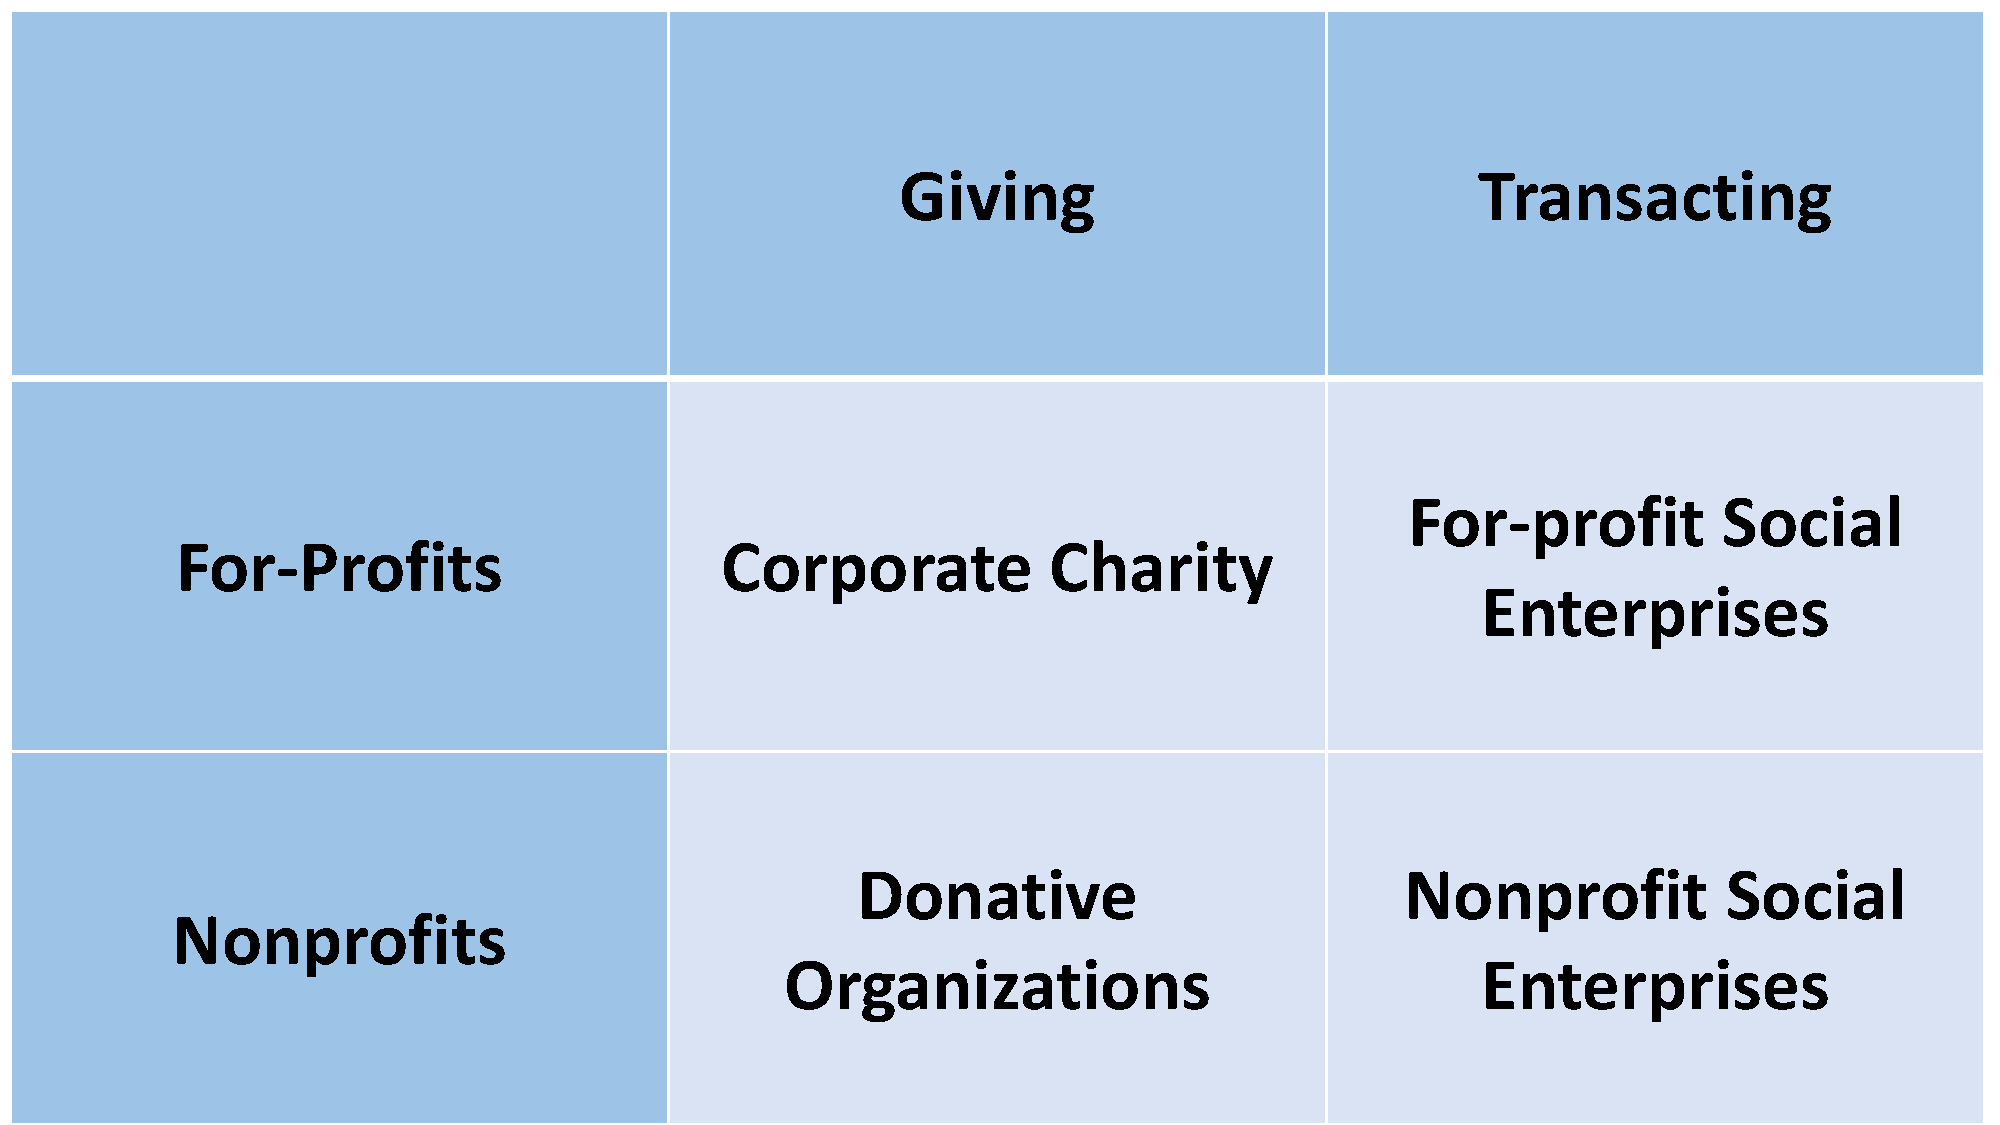
\includegraphics[scale=0.35]{Figure 1.pdf}
\par\end{centering}
\centering{}{\small{}%
\begin{minipage}[t]{0.95\textwidth}%
\begin{spacing}{0}
\end{spacing}
%
\end{minipage}}{\small\par}
\end{figure}

This setup yields three main predictions. First, higher variance in
beneficiaries' abilities and needs increases the value of transacting
with beneficiaries and reduces reliance on giving. Second, and more
importantly, the paper delivers a paradox. The for-profit form arises
when the need for high-quality philanthropy is greatest. When heterogeneity
is high, transacting aligns profit and mission so strongly that the
nonprofit constraint becomes unnecessary. Third, this for-profit commitment
to quality is expressed through lower scale. Absent tax benefits, the
entrepreneur serves fewer beneficiaries rather than expanding philanthropy
through low-quality giving. This implication is also consistent with
anecdotal evidence that social enterprises often remain relatively small.

The legal-form result is a consequence of this choice between giving
and transacting. When beneficiary heterogeneity is low, a nonprofit can improve
quality by weakening the entrepreneur's monetary incentive to underprovide
assistance. When heterogeneity is high, however, transacting itself
creates the information needed for tailored assistance and aligns profit
with mission. In that region, the nondistribution constraint becomes
less important, and the entrepreneur chooses the for-profit form while
serving fewer beneficiaries rather than expanding through low-quality
giving. Thus, the paper's main contribution is not simply that for-profits
and nonprofits coexist. It is to identify a beneficiary-side information
problem that can make transactions with beneficiaries an organizational
solution to low-quality philanthropy.

The paper relates to influential models of socially oriented
firms, including \citet{baron2007}, \citet{besleyGhatak2017},
\citet{deBettigniesRobinson2018}, and \citet{kaulLuo2018}. These
models ask when firms will pursue a given social objective, emphasizing
prosocial preferences, stakeholder demand, employee motivation, or
productive advantages. They take the nature of the socially beneficial
activity as known. This paper instead asks how an organization learns
what effective assistance requires. In many development settings,
beneficiaries' needs are not known ex ante. Transactions with beneficiaries
reveal that information and enable better targeting.

The final part of the paper studies certification. The key implication
is not that certifiers can directly verify impact. Instead, certifiers
may be able to verify a narrower and more realistic object, namely whether
the firm actually transacts with a defined beneficiary group. That
kind of certification can help donors and public funders identify high-quality
organizations without requiring them to observe impact beneficiary by
beneficiary or the entrepreneur's true commitment to costly tailoring.
This intuition is consistent with the emergence of institutions such
as fair trade and community-development certification, which allow
entrepreneurs to commit credibly to beneficiary transactions and, through
them, to higher-quality philanthropy.

The rest of the paper proceeds as follows. \secref{sec:model} presents the
model and articulates the meaning of quality. \secref{sec:analysis} analyzes
the entrepreneur's choice between giving and transacting, the trade-off
between scale and quality, the choice of legal form, and the donor's
decision. \secref{sec:certification} studies certification. \secref{sec:conclusion} concludes by
briefly relating the model to quantity-based notions of philanthropy.
The Appendix contains proofs, and the Online Appendix contains extensions.

\section{Model}\label{sec:model}

The model formalizes a simple targeting problem. An entrepreneur wants
to assist disadvantaged beneficiaries, but she does not initially know
how much assistance each beneficiary needs. She can help beneficiaries
through giving, which can reach many people but must be based on imperfect
information. Alternatively, she can transact with beneficiaries. These
transactions create an opportunity to measure beneficiary-specific abilities
and tailor assistance, but measurement is costly. The central tradeoff is
therefore between scale and targeting.

There is one entrepreneur and a continuum of potential beneficiaries.
Each beneficiary $i$ has ability $a(i)\in[0,\bar{a})$, where $\bar{a}$
is the ability of a standard worker. A lower $a(i)$ means that the
beneficiary needs more assistance. In particular, the assistance needed
to reach the standard-worker level is $\bar{a}-a(i)$. Abilities are
drawn from a distribution with mean $\mathbb{E}(a)$ and variance $Var(a)$.
The entrepreneur knows this distribution but does not initially observe
individual abilities. Beneficiaries come from a fixed pool. Before
transacting, the entrepreneur cannot distinguish their abilities, so
she chooses how many beneficiaries to assist but cannot select them
by type.

The entrepreneur chooses the total scale of philanthropy, denoted by
$n$ and measured by the number of beneficiaries the firm assists.
Of these $n$ beneficiaries, $m$ are served through transactions with
the firm and $g$ are served through giving, so $n=m+g$. Because beneficiaries
form a continuum, $n$, $m$, and $g$ are masses; I refer to them as
numbers throughout.

The entrepreneur also chooses legal form. Let $v$ denote the share
of the firm's monetary payoff that the entrepreneur may appropriate
personally. A for-profit has $v=1$. A nonprofit has $v\in(0,1)$,
a reduced-form representation of the nondistribution constraint. The
analysis first solves the allocation problem for a fixed $v$ and then
compares legal forms.

For concreteness, the formal model uses a work-integration firm. The
firm has a fixed number $w$ of jobs. If it employs $m$ disadvantaged
beneficiaries, the remaining $w-m$ jobs are filled by standard workers,
so $0\leq m\leq w$.\footnote{A similar structure applies to other beneficiary-facing firms. In a fair-trade application, $w$ is the firm's fixed number of supplier relationships, $m$ consists of low-income farmer-suppliers, and the remaining $w-m$ are standard suppliers; revenue depends on the farmers' productivity or input quality after assistance. In microfinance, $w$ is lending capacity and revenue depends on borrowers' ability to repay. For a low-cost service provider, $w$ is the fixed number of customers the firm serves, $m$ consists of low-income customer-beneficiaries, and the remaining $w-m$ are standard customers; revenue depends on customers' ability to pay. In each application, transacting both produces revenue and reveals information relevant to tailoring assistance.}
Beneficiaries served through giving are assisted outside the firm and
do not occupy these jobs.

The timing is:
\begin{itemize}
\item Before choices are made, nature draws beneficiary abilities. The
entrepreneur observes their distribution but not the individual draws.
\item At $t=0$, the entrepreneur chooses legal form, total scale $n$,
and its division between transactions ($m$) and giving ($g=n-m$).
\item At $t=1$, the entrepreneur may incur a cost to measure the abilities
of beneficiaries with whom the firm transacts. She then chooses disbursals,
and payoffs are realized.
\end{itemize}

The cost of measuring the abilities of $m$ beneficiaries is $C(m)$.
The cost function $C$ is increasing, convex, and twice differentiable,
with $C(0)=0$.\footnote{As shown in \secref{oa:linear-cost} of the Online Appendix, the analysis is robust
to a linear cost function.}

For targeting purposes, the key difference between giving and transacting
is what the entrepreneur learns. A disbursal $d(i)\geq0$ is assistance
measured in units of ability. Each unit costs one and raises ability
one-for-one up to $\bar{a}$. Thus, beneficiary $i$ needs the tailored
disbursal $\bar{a}-a(i)$. A smaller disbursal leaves the beneficiary
below $\bar{a}$, while a larger disbursal is wasteful.

If the entrepreneur helps $g\geq0$ beneficiaries through giving, she
does not observe their individual abilities and chooses disbursals
$d^{g}(i)$ based on the distribution of needs.\footnote{The model could in principle allow partial learning through giving,
reflecting limited information acquired through diligence, research,
or screening rather than repeated interaction. I abstract from that
possibility because it would add complexity while providing limited
additional insight into the paper's core mechanism.} If instead she
serves $m$ beneficiaries through transactions, paying $C(m)$ allows
her to observe their abilities before choosing $d^{m}(i)$.

Let $r>1$ be the revenue produced by one unit of worker ability. If
the firm employs only standard workers, revenue is $rw\bar{a}$. If
it instead employs $m$ disadvantaged beneficiaries, realized revenue
is

\[
R(a)=r(w-m)\bar{a}+r\int_{0}^{m}\min\{a(i)+d^{m}(i),\bar{a}\}di.
\]

Thus, a unit of well-targeted assistance costs one but raises revenue
by $r$, increasing net monetary payoff by $r-1>0$.

Donative funding depends on the firm's planned philanthropic scale.
Let $D(n)$ be an increasing, concave, and twice-differentiable donation
schedule, with $D(0)=0$. The concavity of $D(n)$ captures donors' limited
willingness to fund ever-larger scale. This support may come from external
donors, consumer premia, concessionary capital or labor, or the entrepreneur
herself. The schedule also captures the realistic case in which donors
can observe scale more easily than they can assess the quality of disbursals ex ante
\citep{charlesKim2016,coupetSchehl2022}. The entrepreneur takes the
schedule $D(\cdot)$ as given.\footnote{This reduced-form schedule is a tractable simplification of a fuller donor decision in which $U^{D}=Y-D(n)+F(n)$, where $Y$ is donor wealth and $F(n)$ is an increasing, concave benefit from the number of beneficiaries assisted.} \secref{subsec:donor-decision}
later allows donors to care directly about expected quality.

The firm's realized net monetary payoff, $P$, equals realized revenue
plus donative funding, less disbursals through the transaction and
giving channels, and less measurement costs:

\[
P=R(a)+D(n)-\int_{0}^{m}d^{m}(i)di-\int_{0}^{g}d^{g}(i)di-C(m).
\]

Note that the expression for $P$ treats the entrepreneur as incurring
$C(m)$, the cost of measuring the abilities of all $m$ beneficiaries
with whom the firm transacts. I write the problem this way for simplicity.
\lemref{lem:measure-if-transact}, discussed in
\secref{subsec:transacting-giving}, shows that this is without loss
of generality. If the entrepreneur transacts with a beneficiary without
measuring ability, she cannot tailor the disbursal. Assisting that beneficiary
through giving therefore weakly dominates transacting without measurement
because the beneficiary may not receive enough assistance to reach $\bar{a}$,
reducing the firm's expected revenue.

Quality means targeting accuracy, not product quality. Formally,

\[
q=-\int_{0}^{m}\left(d^{m}(i)-(\bar{a}-a(i))\right)^{2}di
-\int_{0}^{g}\left(d^{g}(i)-(\bar{a}-a(i))\right)^{2}di.
\]

Thus, $q\leq0$, and higher $q$ means better targeting. Quality is maximized
at $q=0$, when every beneficiary receives exactly the assistance needed
to reach $\bar{a}$ (that is, $d(i)=\bar{a}-a(i)$). The quadratic loss
treats over-provision and under-provision symmetrically
and provides a tractable measure of targeting accuracy. Quality falls
as a disbursal departs from the beneficiary's need.\footnote{\secref{oa:no-penalty} of the Online Appendix discusses a quality measure with no penalty for waste.}

The entrepreneur's utility is

\begin{equation}
U=vP+\gamma q,
\end{equation}

where $P$ is the firm's net monetary payoff and $\gamma\geq0$ is
the entrepreneur's weight on effective assistance. The analysis below
focuses on social-mission entrepreneurs with $\gamma>0$; the limiting
case $\gamma=0$ corresponds to a purely commercial firm with no weight
on effective assistance. Thus, $\gamma$ captures altruism, reputational
pressure, or both. Unlike \citet{glaeserShleifer2001}, where mission
utility increases with the quantity disbursed, the entrepreneur here
cares about whether assistance is matched to beneficiary need.

Because abilities are unknown at $t=0$, the entrepreneur maximizes expected
utility:

\begin{equation}
\max_{m,g,d^{m},d^{g}}\;v\mathbb{E}[P]+\gamma\mathbb{E}[q]
\quad\mbox{s.t.}\quad n=m+g,\;0\leq m\leq w,\;g\geq0,\;
d^{m}(i),d^{g}(i)\geq0.\label{eq:-1}
\end{equation}

The model's central alignment is now apparent. For a beneficiary the
entrepreneur assists through giving, she must choose $d^{g}(i)$ without
knowing $a(i)$. For a beneficiary with whom the firm transacts, measurement
reveals $a(i)$, and the tailored disbursal $d^{m}(i)=\bar{a}-a(i)$
both raises productive revenue and maximizes targeting quality. Profit
and mission therefore point in the same direction when the firm transacts
with beneficiaries.


\section{Analysis of the Entrepreneur's Choices}\label{sec:analysis}

\subsection{Transacting and Giving as Substitutes}\label{subsec:transacting-giving}

I now solve the entrepreneur's allocation choices for a fixed legal
form $v$. The tradeoff is simple. Giving saves measurement costs but
forces the entrepreneur to use imperfect information. Transacting
requires measurement costs but allows the entrepreneur to tailor assistance
to each beneficiary's need. \secref{app:proofs} provides the formal
proofs for the core lemmas and the main comparative statics.

Start with giving. Because the entrepreneur does not observe individual
ability, all giving beneficiaries are identical from her perspective.
The optimal giving disbursal trades off the monetary cost of paying
more against the quality loss from giving too little or too much. This
gives

\begin{equation}
d^{g*}(i)=\max\left\{0,\bar{a}-\mathbb{E}(a)-\frac{v}{2\gamma}\right\}
\;\;\forall i\in[0,g].\label{eq:2}
\end{equation}

The last term, $\frac{v}{2\gamma}$, reflects the entrepreneur's monetary
incentive to economize on disbursals. This incentive vanishes as
$\gamma\rightarrow\infty.$\footnote{For each giving beneficiary, the relevant first-order condition is
$-v-2\gamma(d-(\bar{a}-\mathbb{E}(a)))=0$, which yields equation
(\ref{eq:2}) when the solution is interior. If the resulting disbursal is nonpositive, the nonnegativity constraint binds and $d^{g*}(i)=0$.} Thus, the more the entrepreneur values effectiveness, the closer
she will set disbursals to the average need of the beneficiaries ($\bar{a}-\mathbb{E}(a)$).
Additionally, the monetary incentive to underprovide vanishes as $v\rightarrow0$,
consistent with the theory that the non-distribution constraint provides
greater incentives to generate more charity.

Unless otherwise stated, the baseline analysis below focuses on the interior
giving region,
\[
\bar{a}-\mathbb{E}(a)>\frac{v}{2\gamma},
\]
where $d^{g*}(i)>0$. When this condition fails, the giving disbursal
is zero. This corner does not affect the measurement logic in the
lemmas below, but it changes the marginal expressions governing scale
and the choice between giving and transacting.

I next solve for the optimal disbursals to the $m$ beneficiaries with
whom the entrepreneur transacts. By incurring $C(m)$, she observes each
beneficiary's ability $a(i)$.
\begin{lem}\label{lem:tailoring}
If the entrepreneur incurs $C(m)$ to observe the abilities of the $m$
beneficiaries with whom she transacts, both her financial and altruistic
incentives lead her to tailor each disbursal to the beneficiary's observed
ability. Thus,
$d^{m*}(i)=\bar{a}-a(i)$ for all $i\in[0,m]$.
\end{lem}
The explanation is that if $d^{m}(i)<\bar{a}-a(i)$, the entrepreneur
loses revenue because the beneficiary performs poorly. Conversely,
if $d^{m}(i)>\bar{a}-a(i)$, the disbursal is wasteful because $a$
cannot exceed $\bar{a}.$ Therefore, increasing disbursals beyond
this amount does not improve the quality of philanthropy.
\begin{lem}\label{lem:measure-if-transact}
Without loss of generality, an entrepreneur who chooses to transact
with beneficiaries incurs measurement costs and tailors disbursals
to their abilities.
\end{lem}
The intuition follows from comparing unmeasured transacting with giving.
Without measurement, the entrepreneur
does not observe $a(i)$ and therefore cannot tailor $d(i)$. Compare
this with assisting the same beneficiary through giving with the same
disbursal. Both choices serve one beneficiary, attract the same donative
funding, and produce the same targeting quality. Under giving, however,
a standard worker remains in production. Under unmeasured transacting,
the beneficiary replaces that worker and may remain less productive
if the disbursal is insufficient to raise her ability to $\bar{a}$.
Unmeasured transacting therefore offers no targeting advantage and
may reduce revenue, so giving weakly dominates it.

Having characterized the optimal disbursal under each channel, I now
consider how the entrepreneur allocates beneficiaries between transacting
and giving. For the comparative statics below, I focus on a finite,
unique interior solution with positive measurement and nonbinding production
capacity.\footnote{Specifically, I assume that $C$ is strictly convex, $D$ is strictly concave with $\lim_{n\rightarrow\infty}D'(n)=0$, and the relevant first-order conditions have solutions. I also assume that $w$ is sufficiently large that the capacity constraint does not bind. If capacity binds, transacting is capped at $m^{*}=w$. If measurement is not worthwhile at $m=0$, the pure-giving corner applies, as discussed in \secref{subsec:legal-form-effects}.}
The entrepreneur can increase total scale $n$ either by raising $m$
or by raising $g$. Raising $m$ expands scale through
transactions. The entrepreneur receives the marginal donation, pays
the expected disbursal, and pays the marginal measurement cost. Raising
$g$ expands scale through giving. The entrepreneur receives the marginal
donation and pays the expected disbursal, but also bears the expected
quality loss from untailored assistance. For a candidate allocation
$(n',m',g')$ in the maintained interior region, substituting the optimal
disbursal rules into equation (\ref{eq:-1}) gives

\begin{equation}
\begin{aligned}
&v\left(r\cdot w\cdot\overline{a}+D(n')-C(m')-n'\left(\bar{a}-\mathbb{E}(a)\right)\right)\\
&\qquad -g'\cdot\gamma Var(a)+\frac{v^{2}g'}{4\gamma}
\end{aligned}
\label{eq:3}
\end{equation}

If $n$ is increased by raising $m$, the marginal change in expected
utility is
\[
v\left(D'(n')-\left(\bar{a}-\mathbb{E}(a)\right)-C'(m')\right).
\]
If $n$ is increased by raising $g$, the marginal change is
\[
v\left(D'(n')-\left(\bar{a}-\mathbb{E}(a)\right)\right)-\gamma Var(a)+\frac{v^{2}}{4\gamma}.
\]
Define
\[
S(v)\equiv\frac{\gamma}{v}Var(a)-\frac{v}{4\gamma}.
\]
$S(v)$ is the marginal advantage of measured transacting over giving,
expressed in monetary-payoff units. The entrepreneur will expand through
transactions rather than giving only if
\[
C'(m')<S(v)
\quad\text{and}\quad
C'(m')<D'(n')-\left(\bar{a}-\mathbb{E}(a)\right).
\]
The first condition requires the targeting benefit from measurement
to exceed its marginal cost. The second requires marginal donative
funding, net of the expected disbursal, to cover that cost.
If the first inequality fails, the entrepreneur raises $g$ only when
the marginal return from giving is positive. If neither channel has
a positive marginal return, she stops expanding.

At an interior optimum, one of two limits stops expansion through transactions.
The targeting limit, $m_{T}^{*}$, is reached when

\begin{equation}
C'(m_{T}^{*})=S(v)<D'(m_{T}^{*})-\left(\bar{a}-\mathbb{E}(a)\right).\label{eq:4}
\end{equation}
Beyond this point, additional measurement costs more than its targeting
benefit. The funding limit, $m_{F}^{*}$, is reached when

\begin{equation}
C'(m_{F}^{*})=D'(m_{F}^{*})-\left(\bar{a}-\mathbb{E}(a)\right)<S(v).\label{eq:5}
\end{equation}
Beyond this point, marginal donative funding net of the expected disbursal
no longer covers measurement cost.

These conditions show that transacting with beneficiaries is preferable
when $Var(a)$ is large, reflecting the informational advantage of
social enterprises. Conversely, giving is preferable when $Var(a)$
is small. Similarly, transacting is favored when the entrepreneur
has a high regard for the quality of philanthropy ($\gamma$), while giving is more suitable when $\gamma$
is low. Thus, the entrepreneur internalizes the need to tailor disbursals
when the variance in abilities is greater and she places higher value
on subsidy effectiveness.

If the funding limit binds first, the entrepreneur serves beneficiaries
only through transactions, so
\[
m^{*}=n^{*}=m_{F}^{*},\qquad g^{*}=0.
\]
If the targeting limit binds first, she sets $m^{*}=m_{T}^{*}$ and
increases $n$ through giving until
\[
D'(n_{T}^{*})=S(v)+\left(\bar{a}-\mathbb{E}(a)\right).
\]
This implies that $n_{T}^{*}$ decreases as $Var(a)$ and $\gamma$
increase. Conversely, $m_{T}^{*}$ increases with $Var(a)$ and $\gamma$
because $C(m)$ is strictly convex over the relevant range.
\lemref{lem:mapping} and \propref{prop:comparative-statics} summarize these comparative statics.
\begin{lem}\label{lem:mapping}
In the mixed regime, there exists a one-to-one mapping between $m^{*}$
and $n^{*}$, between $m^{*}$ and $g^{*}$, and between $g^{*}$ and
$n^{*}$.
\end{lem}
\begin{prop}\label{prop:comparative-statics}
Under the maintained interior and regularity conditions:
\textbf{(A)} When the variance in abilities ($Var(a)$) is high and
the entrepreneur has high regard for quality ($\gamma$ is high),
she transacts with a larger number of beneficiaries ($m$). Conversely,
when $Var(a)$ and $\gamma$ are low, she is more likely to engage
in giving to a greater number of beneficiaries ($g$). 

\textbf{(B)} When $Var(a)$ and $\gamma$ are small, such that $m^{*}=m_{T}^{*}$,
where $C'(m_{T}^{*})=S(v)<D'(m_{T}^{*})-\left(\bar{a}-\mathbb{E}(a)\right)$,
the total number of beneficiaries the entrepreneur chooses to assist
($n^{*}$) decreases with the number transacted with ($\frac{\partial n^{*}}{\partial m^{*}}(Var(a),\gamma)<0$)
and increases with the number helped through giving ($\frac{\partial n^{*}}{\partial g^{*}}(Var(a),\gamma)>0$). 

\textbf{(C)} When $Var(a)$ and $\gamma$ are large, such that $m^{*}=m_{F}^{*}$,
where $C'(m_{F}^{*})=D'(m_{F}^{*})-\left(\bar{a}-\mathbb{E}(a)\right)<S(v)$,
the total number of beneficiaries the entrepreneur chooses to assist
($n_{F}^{*}$) is equal to the number of beneficiaries the entrepreneur
transacts with ($m_{F}^{*}$), and the entrepreneur does not engage
in giving ($g_{F}^{*}=0$).

\textbf{(D)} In the pure-transacting regime, $n^{*}=m^{*}=m_{F}^{*}$
and $g^{*}=0$, so every assisted beneficiary is served through a transaction.
\end{prop}
This proposition highlights the trade-off faced by social entrepreneurs
between scale and the quality of philanthropy. The scale of philanthropy is determined
by $n$. Quality is defined as $q=-\int_{0}^{n}\left(d(i)-(\bar{a}-a(i))\right)^{2}di,$
where misallocation of disbursals reduces the quality of philanthropy.
Under the maintained interior condition, \lemref{lem:tailoring} and equation (\ref{eq:2}) imply that expected quality is $\mathbb{E}\left[q\right]=-g^{*}\left(Var(a)+\frac{v^{2}}{4\gamma^{2}}\right)$.
Maximum philanthropic quality is achieved when the entrepreneur engages exclusively
in transacting ($g^{*}=0$), resulting in $\mathbb{E}\left[q\right]=0$.
When the entrepreneur mixes transacting and giving, $\frac{\partial n^{*}}{\partial m^{*}}(Var(a),\gamma)<0$
and $\frac{\partial n^{*}}{\partial g^{*}}(Var(a),\gamma)>0$. For
very small $Var(a)$, the need for transacting is low. As $Var(a)$
and $\gamma$ increase, both the need for tailoring and the entrepreneur's
regard for quality are higher, leading to larger $m^{*}$ and smaller
$n^{*}$. For sufficiently high $Var(a)$, expected quality increases
with $\gamma$, such that $\mathbb{E}\left[q\right]\rightarrow0$
as $n^{*},m^{*}\rightarrow m_{F}^{*}=n_{F}^{*}$.\footnote{The relationship between expected quality and $Var(a)$ is defined
as $\frac{\partial\mathbb{E}\left[q\right]}{\partial Var(a)}=-\frac{\partial g^{*}}{\partial Var(a)}\left(Var(a)+\frac{v^{2}}{4\gamma^{2}}\right)-g^{*}$.
This derivative may be negative or positive. Using the condition that
$D'(n_{T}^{*})=\left(\bar{a}-\mathbb{E}(a)\right)+S(v)$,
it can be shown that $g^{*}\left(Var(a)\right)$ is a declining convex
function of $Var(a)$, and $\frac{\partial g^{*}}{\partial Var(a)}\left(Var(a)\right)<0$
is an increasing concave function. For high values of $Var(a)$, $\frac{\partial\mathbb{E}\left[q\right]}{\partial Var(a)}>0$.
By contrast, expected quality always increases with $\gamma.$ Specifically,
$\frac{\partial\mathbb{E}\left[q\right]}{\partial\gamma}=-\frac{\partial g^{*}}{\partial\gamma}\left(Var(a)+\frac{v^{2}}{4\gamma^{2}}\right)+\frac{g^{*}v^{2}}{2\gamma^{3}}>0$,
because $\frac{\partial g^{*}}{\partial\gamma}<0$ .}
\begin{cor}\label{cor:quality-scale}
When $n^{*}=m^{*}=m_{F}^{*}$, the expected quality of philanthropy
is maximized. Conversely, when $m^{*}=m_{T}^{*}$ and $Var(a)$
is sufficiently high, the expected quality of philanthropy increases
as $m^{*}\left(Var(a),\gamma\right)$ rises and $n^{*}\left(Var(a),\gamma\right)$
declines.
\end{cor}
Accordingly, there is a trade-off between expected quality of philanthropy and scale
(See \exampleref{ex:oa-tradeoff} in \secref{oa:examples} of the Online Appendix). Entrepreneurs
who prioritize effectiveness tend to focus on a smaller number of
beneficiaries, while those operating in environments with lower information
asymmetries and relying on standardized disbursals are more likely
to prioritize scale. Thus, some social enterprises achieve broader
reach at the expense of quality, whereas others concentrate on delivering
tailored support to a more limited group. For example, large corporations
that market fair-trade products may achieve greater scale while relying
more on standardized support. In contrast, smaller sourcing organizations
may focus on repeated transactions with a more limited number of disadvantaged
farmers and on more tailored support \citep{eldar2017}.

\subsection{The Effect of Legal Form on the Scale and Quality of Philanthropy}\label{subsec:legal-form-effects}

To evaluate the effect of legal form on the scale and quality of philanthropy,
I consider the choices made by for-profit and nonprofit entrepreneurs.
Recall that for nonprofits, $v<1$, and for for-profits, $v=1$. For
this analysis, I assume $v<1$ (rather than $v\leq1$). The subscripts
$fp$ and $np$ denote the choices of for-profit and nonprofit entrepreneurs,
respectively. The key effect of a lower $v$ is simple: it lowers
the entrepreneur's private monetary payoff, so the quality term becomes
relatively more important. A nonprofit entrepreneur is therefore willing
to bear higher measurement costs; specifically,
$S(v)>S(1)$
(see equation (\ref{eq:4})). As illustrated in Figure 2, three main
cases arise depending on the levels of $\gamma$ and $Var(a)$:

$\;$

\noindent\begin{minipage}[t]{1\columnwidth}%
\begin{center}
Figure 2: \textbf{Legal Form and the Entrepreneur's Choice between
Transacting and Giving}
\par\end{center}
\begin{center}
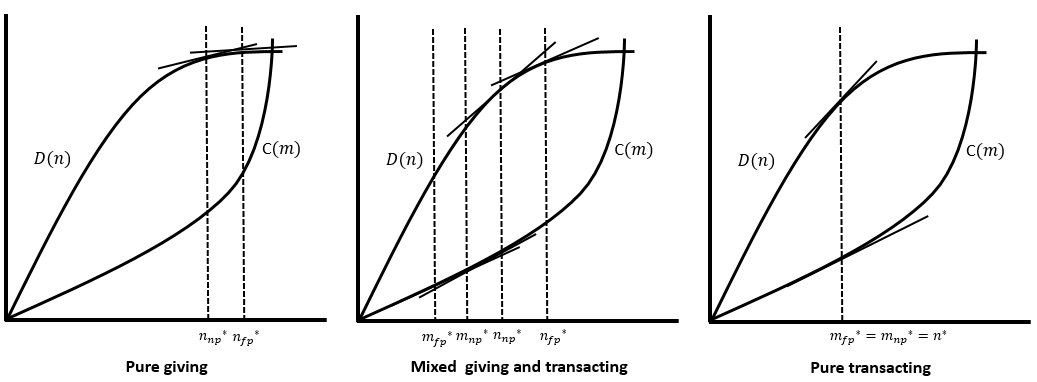
\includegraphics[scale=0.45]{Figure 2.PNG}
\par\end{center}
\begin{center}
\begin{minipage}[t]{0.95\textwidth}%
\begin{spacing}{0}
{\footnotesize This figure illustrates the three key outcomes of the
entrepreneur's decision-making process in selecting $m$ and $n$,
depending on whether the firm operates as a nonprofit ($np$) or a
for-profit ($fp$). }
\end{spacing}
%
\end{minipage}
\par\end{center}%
\end{minipage}

$\;$

\textbf{Case 1. Pure Giving:} Pure giving occurs when measurement
is never worth its cost. Formally, the targeting limit
in equation (\ref{eq:4}) is not satisfied for any $m$. Suppose
$C'(0)>S(v)$.
This implies that when $Var(a)$ is low or $\gamma$ is small, the
nonprofit entrepreneur will form a donative organization ($m_{np}^{*}=0$).
Similarly, the for-profit entrepreneur will engage in pure giving
($m_{fp}^{*}=0$) because $S(v)>S(1)$,
and $C(m)$ is convex. Setting $m^{*}=0$ and solving equation (\ref{eq:-1}),
the number of beneficiaries served by donative organizations is determined
by $D'(n_{np}^{*})=\bar{a}-\mathbb{E}(a)+S(v).$
For for-profits, $D'(n_{fp}^{*})=\bar{a}-\mathbb{E}(a)+S(1)<D'(n_{np}^{*})$.
Since $D(n)$ is concave, this implies that $n_{np}^{*}=g_{np}^{*}<g_{fp}^{*}=n_{fp}^{*}$.
While for-profits give to more beneficiaries, nonprofits provide higher
per-capita disbursals because $d_{np}^{g*}=\bar{a}-\mathbb{E}(a)-\frac{v}{2\gamma}>d_{fp}^{g*}=\bar{a}-\mathbb{E}(a)-\frac{1}{2\gamma}$.
As a result, the expected quality of philanthropy by nonprofits is
higher: $\mathbb{E}\left[q_{np}\right]=-g_{np}^{*}\left(Var(a)+\frac{v^{2}}{4\gamma^{2}}\right)>-g_{fp}^{*}\left(Var(a)+\frac{1}{4\gamma^{2}}\right)=\mathbb{E}\left[q_{fp}\right]$.

\textbf{Case 2. Mixed Giving and Transacting:} Mixed giving and transacting
occurs when measurement is useful for some beneficiaries but not for
all additional scale. Suppose that $C'(m^{*})=S(1)=\gamma Var(a)-\frac{1}{4\gamma}$
satisfies the targeting limit for the for-profit
firm (see equation (\ref{eq:4})). This means that the for-profit
entrepreneur will continue to increase $n$ until $n$ satisfies the
equation $D'(n_{fp}^{*})=\bar{a}-\mathbb{E}(a)+S(1)$.
Thus, the entrepreneur will mix transacting with beneficiaries and giving
to them. At $m=m_{fp}^{*}$, the nonprofit entrepreneur will continue
to increase the number of beneficiaries she transacts with because $C(m)$
is convex, implying $m_{np}^{*}>m_{fp}^{*}.$ The nonprofit entrepreneur
will increase $n$ up to $n_{np}^{*}<n_{fp}^{*}$, as in Case 1.\footnote{I assume the nonprofit also mixes between giving and transacting,
although it is possible that the nonprofit will engage exclusively
in transacting if the funding limit is reached.} It follows that $g_{fp}^{*}>g_{np}^{*}\geq0$ because $n=m+g$. Accordingly,
$\mathbb{E}\left[q_{np}\right]>\mathbb{E}\left[q_{fp}\right]$.

\textbf{Case 3. Pure Transacting:} Pure transacting occurs when beneficiary
heterogeneity and the entrepreneur's concern for quality are high
enough that the entrepreneur avoids giving altogether. The funding
limit in equation (\ref{eq:5}) is then reached,
i.e., $C'(m^{*})=D'(m^{*})-\left(\bar{a}-\mathbb{E}(a)\right)$.
As $D(n)$ is concave, the marginal income from donations decreases
with $n$, and at high levels of $\gamma Var(a)$, the funding limit
will be reached. When the informational advantages
are significant, social enterprises focus exclusively on transacting.
Importantly, the funding limit is identical
for both for-profit and nonprofit firms because it does not depend
on $v$. Consequently, $m_{np}^{*}=m_{fp}^{*}=n_{np}^{*}=n_{fp}^{*}$,
and $g_{np}^{*}=g_{fp}^{*}=0$. Moreover, since $d_{np}^{m*}=d_{fp}^{m*}=\bar{a}-a(i)$
(per \lemref{lem:tailoring}), $\mathbb{E}\left[q_{np}\right]=\mathbb{E}\left[q_{fp}\right]=0.$
Accordingly, the quality of philanthropy for both for-profit and nonprofit
firms is maximal.
\begin{prop}\label{prop:legal-form-effects}
When $Var(a)$ and $\gamma$ are medium or low, a nonprofit is expected
to produce higher-quality philanthropy, measured as subsidy-effectiveness
($\mathbb{E}\left[q_{np}\right]>\mathbb{E}\left[q_{fp}\right]$),
while a for-profit produces philanthropy at a greater scale than a
nonprofit ($n_{np}^{*}<n_{fp}^{*}$). When $Var(a)$ and $\gamma$
are high, such that the entrepreneur engages exclusively in transacting
with beneficiaries, nonprofits and for-profits produce the same quality
($\mathbb{E}\left[q_{np}\right]=\mathbb{E}\left[q_{fp}\right]$) and
scale ($n_{np}^{*}=n_{fp}^{*}$ and $g_{np}^{*}=g_{fp}^{*}=0$).
\end{prop}
This result shows that when informational asymmetries are not substantial,
nonprofit entrepreneurs do not necessarily produce more charity than
for-profits but instead deliver higher-quality philanthropy. However,
when informational asymmetries are substantial, entrepreneurs already
have strong incentives to gather information about beneficiaries\textquoteright{}
abilities and tailor disbursals accordingly. In such cases, where
all disbursals are tied to transactions and measurement, the nonprofit
form is no longer necessary to ensure effectiveness. This finding
reinforces the view that for-profits can be just as effective as nonprofits
in delivering high-quality philanthropy \citep{haber2016,pallotta2022}.
\begin{cor}\label{cor:no-info}
Without information asymmetries (i.e., when $a(i)$ is observable
for every $i$), social enterprises are redundant: there is an optimum
with $m^{*}=0$. A for-profit produces philanthropy at a greater
scale than a nonprofit ($n_{np}^{*}<n_{fp}^{*}$), and a nonprofit
provides higher-quality philanthropy than a for-profit ($q_{np}>q_{fp}$).
\end{cor}
When there are no information asymmetries, there is no benefit to
measurement because the entrepreneur already observes $a$. Social
enterprises emerge primarily in development contexts, where entrepreneurs
are not able to observe the abilities of disadvantaged groups, such
as productivity or creditworthiness. In contrast, in other social
contexts, such as providing assistance to the destitute, information
asymmetries are less significant, and the need for tailoring is correspondingly
lower.

\subsection{The Entrepreneur's Choice of Legal Form}\label{subsec:legal-form-choice}

To determine which legal form the entrepreneur will choose, I compare
the entrepreneur's utility from forming a nonprofit ($U_{np}^{E}$)
with that of forming a for-profit ($U_{fp}^{E}$). The ex ante utility
of the nonprofit entrepreneur is defined by equation $\left(\ref{eq:3}\right)$,
with $n'$ and $m'$ replaced by $n^{*}$ and $m^{*}$, respectively.
For the for-profit entrepreneur, the utility is identical except that
$v=1.$ This analysis assumes that nonprofits receive no tax benefits
and that the project's net monetary component is nonnegative at the
relevant allocations.

The simplest case arises when the entrepreneur engages exclusively
in transacting with the beneficiaries (Case 3 in \secref{subsec:legal-form-effects}), where
$m_{fp}^{*}=m_{np}^{*}$ and $g_{fp}^{*}=g_{np}^{*}=0$. In this scenario,
$U_{np}^{E}=vU_{fp}^{E}$, making the for-profit form the clear choice.
The nonprofit form is redundant, as it imposes restrictions without
affecting the scale or quality of philanthropy. When the entrepreneur
mixes transacting and giving (Case 2 in \secref{subsec:legal-form-effects}), the nonprofit
produces higher-quality philanthropy, while the for-profit achieves
greater scale. Nonetheless, the entrepreneur still selects the for-profit
form because:

\begin{equation}
U_{fp}^{E}=r\times w\times\bar{a}+D\left(n_{fp}^{*}\right)-C(m_{fp}^{*})-n_{fp}^{*}\left(\bar{a}-\mathbb{E}(a)\right)-g_{fp}^{*}\gamma Var(a)+g_{fp}^{*}\frac{1}{4\gamma}>\label{eq:6}
\end{equation}
\[
r\times w\times\bar{a}+D\left(n_{np}^{*}\right)-C(m_{np}^{*})-n_{np}^{*}\left(\bar{a}-\mathbb{E}(a)\right)-g_{np}^{*}\gamma Var(a)+g_{np}^{*}\frac{1}{4\gamma}>
\]

\[
v\left(r\times w\times\bar{a}+D\left(n_{np}^{*}\right)-C(m_{np}^{*})-n_{np}^{*}\left(\bar{a}-\mathbb{E}(a)\right)\right)-g_{np}^{*}\gamma Var(a)+g_{np}^{*}\frac{v^{2}}{4\gamma}=U_{np}^{E}.
\]

The first inequality holds because the for-profit entrepreneur maximizes
utility by choosing optimal allocations for the for-profit form. The
second inequality holds because $v<1$ and the nonprofit's net monetary
component is nonnegative by assumption. From equation $\left(\ref{eq:6}\right)$,
the for-profit form also dominates the nonprofit form when the entrepreneur
engages solely in giving (Case 1 in \secref{subsec:legal-form-effects}), with $n_{fp}^{*}=g_{fp}^{*}$,
$n_{np}^{*}=g_{np}^{*}$, and $C(m_{fp}^{*})=C(m_{np}^{*})=C(0)=0$.
Thus, even though nonprofits may produce higher-quality philanthropy
than for-profits (see \propref{prop:legal-form-effects}), the entrepreneur still chooses
the for-profit form. 
\begin{prop}\label{prop:legal-form-choice}
The entrepreneur chooses the for-profit form if: (a) there are information
asymmetries regarding beneficiaries' abilities ($a$); (b) quality
is defined as subsidy-effectiveness ($q=-\int_{0}^{n}(d(i)-(\bar{a}$
$-a(i)))^{2}di$); (c) donation amounts increase concavely with the scale
of philanthropy ($n$); and (d) the scale of philanthropy is observable
ex ante. 
\end{prop}
Accordingly, even when the nonprofit delivers higher-quality philanthropy
(see Cases 1 and 2 in \secref{subsec:legal-form-effects}), the for-profit still attracts
more donations ($D(n_{fp}^{*})>D(n_{np}^{*})$). This occurs because
the for-profit assists more beneficiaries ($n_{fp}^{*}>n_{np}^{*}$)
and spends less on measurement (because $m_{fp}^{*}<m_{np}^{*}$),
placing less emphasis on quality than the nonprofit. Although reputational
costs from misallocated disbursals rise with scale, the for-profit
is more willing to tolerate them in order to raise additional donations
(see \exampleref{ex:oa-legal-form} in \secref{oa:examples} of the Online Appendix).

\propref{prop:legal-form-choice} relies on two assumptions. The first is that donations to
nonprofits are not tax-deductible. Tax deductibility increases nonprofit
donations and can incentivize entrepreneurs to choose the nonprofit
form. Without tax exemptions, nonprofits may struggle to raise funds
even if they provide higher-quality philanthropy. By contrast, large
charitable arms of for-profit firms frequently attract substantial
capital, via consumer premiums or investors accepting lower
returns, even amid concerns over the quality of for-profit
philanthropy \citep[see][]{masulisReza2015}.\footnote{The effect of tax deductibility on philanthropy quality is more nuanced.
As shown in \secref{oa:tax-deductions} of the Online Appendix, tax benefits induce
entrepreneurs to scale up. When the tax incentive is modest, the entrepreneur
increases scale by transacting with more beneficiaries, thereby maintaining
high quality. However, excessively large tax benefits may encourage
ineffective giving, thereby reducing quality.} The second is that scale
is observable ex ante, so donors can condition support on planned scale.
\secref{subsec:donor-decision} shows that once donors also care directly about expected quality,
the for-profit result survives in the pure-transacting region, but
the legal-form comparison can become ambiguous when some giving remains.

\subsection{The Donor's Decision}\label{subsec:donor-decision}

The baseline model keeps the donor side deliberately tractable so that
the core mechanism is easy to see. When donors base funding only on
scale, an explicit donor problem adds little beyond a microfoundation
for $D(n)$. The reduced-form donation schedule already captures the
idea that larger promised scale attracts more support. Once donations
are summarized by $D(n)$, the entrepreneur fully internalizes how funding
responds to scale, so modeling the donor's optimization separately
does not change the choice between giving and transacting or the baseline
choice of legal form.

The more interesting case arises when donors care directly about expected
quality of philanthropy. \secref{oa:donors-quality} of the Online Appendix develops
this donor problem formally. The discussion here lays out the intuition.
Once donors care about expected quality,
they must form beliefs about how much ineffective giving the entrepreneur
is willing to tolerate. In this model, that depends on $\gamma$, the
weight the entrepreneur places on the quality of disbursals. The donor
therefore funds the enterprise based on beliefs over $\gamma$ rather
than on scale alone.\footnote{This informational problem is not unique
to the for-profit form. Donors also cannot observe the entrepreneur's
altruism when the enterprise is organized as a nonprofit. In \citet{glaeserShleifer2001},
by contrast, the analogous altruism parameter $b$ is assumed to be
observable.} Donor concern
for the quality of philanthropy makes ineffective giving harder to
finance and therefore strengthens the case for transactions with beneficiaries.

The extension can be summarized as follows.
\begin{prop}\label{prop:donor-quality}
Suppose donors care directly about expected quality of philanthropy.
If $Var(a)$ and the donor's expected level of altruism, $\mathbb{E}\left[\gamma\right]$,
are high enough that the equilibrium is pure transacting, both legal
forms avoid giving, the quality of philanthropy is maximal under either
form, and the entrepreneur prefers the for-profit form absent tax
benefits. Outside this region, when some giving remains, donor concern
for expected quality can weaken or overturn the baseline preference
for the for-profit form, so a nonprofit may be chosen.
\end{prop}

This is the sense in which the paradox survives: even when donors
care directly about expected quality, the for-profit remains preferred
in the high-information-asymmetry region where the entrepreneur relies
entirely on transactions with beneficiaries.

This high-information-asymmetry case is substantively important. In
many development settings, the central problem is not simply how much
assistance to provide, but how to learn enough about beneficiaries'
abilities and needs to improve employment opportunities, raise the
productivity of farmers, or expand access to capital \citep{eldar2017}. In those settings,
transactions with beneficiaries are especially valuable because they
generate the information needed for effective assistance.

When some giving remains, however, donor concern for expected quality
no longer yields a sharp legal-form ranking. The nonprofit may transact with
more beneficiaries, but it may also attract more total funding and
operate at larger scale. Because expected quality in the mixed region
depends on residual giving, higher $m_{np}$ does not by itself imply
higher-quality philanthropy if $n_{np}$ rises as well. The result is
therefore more qualified: donor concern for quality can weaken
or overturn the baseline legal-form ranking in this intermediate region,
even though it does not overturn the central paradox in the high-variance
pure-transacting case.

\section{Certification of Transactions with Beneficiaries}\label{sec:certification}

As \corref{cor:quality-scale} shows, the highest-quality outcome
in the model is the pure-transacting outcome: when the entrepreneur
relies entirely on transactions with beneficiaries, expected quality
is maximized, but further expansion through giving would reduce quality.
This creates a scaling challenge, which is consistent with recurring
concerns about the difficulty social enterprises face in scaling their
impact. In the observable-scale benchmark,
however, certification is not yet needed. As \secref{oa:donors-quality}
of the Online Appendix shows, even when donors care directly about
expected quality, observable scale lets them infer the implied quality
of philanthropy in equilibrium. Certification becomes relevant only
when donors can no longer infer the entrepreneur's true $\gamma$,
and therefore expected quality, from observable scale.

This observability problem is developed formally in \secref{oa:scale-unobservable}
of the Online Appendix. Once scale is not verifiable ex ante, donors
cannot accurately infer the entrepreneur's true $\gamma$ and instead
base funding decisions on the expected level of altruism, $\mathbb{E}\left[\gamma\right]$.
This creates a risk that donors overestimate altruism ($\gamma<\mathbb{E}\left[\gamma\right]$),
leading to lower-than-expected philanthropic quality, or underestimate
altruism ($\gamma>\mathbb{E}\left[\gamma\right]$), leading them to
underfund high-quality organizations and keep them at inefficiently
low scale.\footnote{A similar problem would arise if donors could not observe
the entrepreneur's measurement technology or cost of transacting, $C(m)$.
Donors may then be reluctant to fund an entrepreneur who has developed
an unusually effective measurement technology that allows her to transact
with many beneficiaries at low cost if that technology is not observable
to them. Conversely, if donors overestimate the entrepreneur's measurement
technology, they may overfund an organization that cannot in fact deliver
high-quality philanthropy at the expected scale.} The problem matters even if donors care only about
scale, because in the main model they still face reputational costs
when philanthropy is ineffective. It is exacerbated when donors care
directly about expected quality.

The analysis in this paper offers a simple certification mechanism.
The certifier does not verify philanthropic quality directly, which
is unknown ex ante. Instead, the certifier verifies the entrepreneur's
commitment to transact with $m^{*}$ beneficiaries. Certification
is typically conducted by a government agency or a nonprofit organization.\footnote{Alternatively, a nonprofit may own a for-profit or contract with one,
requiring it to transact with beneficiaries \citep{eldar2017,eldarOrberg2026}. These mechanisms are most practical when the nonprofit
is the donor and can use its ownership to control the entrepreneur's
choices. In contrast, certification is suited to a broader donor base,
including consumers and private investors \citep[see][]{eldar2020}.} Beneficiaries may be defined by income, unemployment status, geographic
location, or lack of access to technology.\footnote{For a discussion of how beneficiaries can be classified and the challenges
involved in doing so, see \citet{eldar2020}.} A well-known example is fair trade certification, which ensures firms
source products from disadvantaged farmers in developing countries.
Through certification, the entrepreneur commits to transact with $m$
beneficiaries. She will do so if donations compensate her for measurement
and disbursal costs, so $D'(m^{*})\geq C'(m^{*})+\left(\bar{a}-\mathbb{E}(a)\right)$.
The quality of philanthropy is then maximized ($\mathbb{E}\left[q\right]=0$)
because the entrepreneur, incentivized by revenue, sets $d_{i}^{m}=\bar{a}-a(i)$
for every transacted beneficiary. Failing to do so reduces revenue
(see \lemref{lem:tailoring}). The donor sets the donation amount according
to the donor's own value of scale, so $D'(m^{*})=F'(m^{*})$, where
$F$ is the donor's benefit from beneficiaries assisted.
Together, these conditions imply that certified scale must satisfy
$F'(m^{*})\geq C'(m^{*})+\left(\bar{a}-\mathbb{E}(a)\right)$. 

Certification changes what donors need to infer. Without certification,
donors who care about quality may read small scale as a signal that
the entrepreneur cares about the quality of philanthropy, while donors
who care mainly about scale may still be unable to verify whether
promised beneficiary transactions will actually occur. With certification,
donors no longer need to rely on scale alone because the certified
entrepreneur is committed to transact with a defined beneficiary group,
and those transactions themselves create the information needed for
correct tailoring.

This mechanism is narrower than direct impact certification. The certifier
verifies transactions with beneficiaries, not the entire impact process.
That interpretation is broadly consistent with institutions such as
fair trade and CDFI certification, even though the model is not meant
as a literal description of every detail of those programs. Fair trade
certification verifies sourcing from certified producers, while CDFI
certification verifies service to underserved communities and unlocks
subsidized capital \citep{dragusanuGiovannucciNunn2014,dragusanuMonteroNunn2022,frbny2023}. In both cases, certification verifies a limited
mission-related activity rather than impact itself, which is the narrower
point captured by the model.

It is important to emphasize that certification for verifying quality
through giving ($g$) is largely a futile mechanism. Even if a legal
mechanism certifies that the entrepreneur gives to beneficiaries,
donors cannot accurately predict the actual quality of philanthropy
because neither the donor nor the entrepreneur knows $a$. And if scale
is not observable, such that donors cannot infer $\gamma$, donors cannot
infer the giving rule or the actual disbursals the entrepreneur will
give. As a result,
certifying giving is impossible without a technology that measures
actual disbursals to individual beneficiaries. But such measurement,
essentially general impact assessment, is typically prohibitively costly.
In contrast, when the entrepreneur is certified as transacting with
beneficiaries, she has a market platform and financial incentives
to allocate effective, tailored disbursals (see \lemref{lem:measure-if-transact}). Certification
of transacting does not require monitoring actual disbursals because
the entrepreneur who submits to certification has an economic stake
in incurring $C(m^{*})$ to learn the true $a$ and allocate optimal
disbursals. Thus, certification ensures maximal quality without general
impact assessment by aligning entrepreneurial incentives with optimal
philanthropy.
\begin{prop}\label{prop:certification}
Certification of the number of beneficiaries the entrepreneur transacts
with ($m$) enables donors to ensure that entrepreneurs provide maximal
quality philanthropy ($\mathbb{E}\left[q\right]=0$). In contrast,
certification of the number of beneficiaries the entrepreneur gives
to ($g$) cannot assure donors of philanthropic quality due to information
asymmetries regarding the true abilities of beneficiaries ($a$). 
\end{prop}
Certification may be implemented by private actors, such as the Fair
Trade Labeling Organization, or embedded in public programs that subsidize
social enterprises, such as CDFIs. When embedded in a public program,
the government plays a dual role, as both certifier and
donor. As a donor, the government faces the same challenge as other
donors who care about the quality of philanthropy, but it also possesses
the legal authority and institutional tools to certify social enterprises.
CDFIs, for example, are certified and subsidized by the CDFI Fund,
a government agency, as financial institutions serving low-income
communities. Similarly, several European legal regimes certify firms
that employ disadvantaged workers and entitle them to subsidies \citep{eldar2020}. Such certifications enable for-profit firms to credibly commit
to delivering high-quality philanthropy.

The certification system also enables the government to set the optimal
level of subsidies. These subsidies are conditional on the firm transacting
with a specified number of beneficiaries. As long as the subsidy amount
is equal to or greater than $C(m^{*})+m^{*}\left(\bar{a}-\mathbb{E}(a)\right)$,
the entrepreneur will agree to transact with $m^{*}$ beneficiaries.
Alternatively, the subsidy may take the form of a tax credit, which
in this model functions like a tax deduction by reducing the cost
of donations for private donors.\footnote{The tax deduction is incorporated by multiplying $D(n)$ by a scalar
($\lambda>1$) in Equation $\left(\ref{eq:-1}\right)$. The tax credit
required to incentivize the entrepreneur to transact with $m^{*}$ beneficiaries
is given by $\lambda=\frac{C'(m^{*})+\left(\bar{a}-\mathbb{E}(a)\right)}{D'(m^{*})}$.} In this setting, the donors are often investors who provide capital
at below-market rates. For example, the New Markets Tax Credit Program
offers investors in CDFIs a tax credit equal to 39\% of the original
investment. Unlike such targeted tax credits, which are conditional
on transacting with $m$ beneficiaries, a general
tax deduction for donations to nonprofits may actually encourage ineffective
giving (see \secref{oa:tax-deductions} of the Online Appendix). Accordingly, to facilitate
subsidized funding to social enterprises, policymakers should prioritize
the development of certification mechanisms for firms that transact
with their beneficiaries.

\section{Conclusion}\label{sec:conclusion}

Recent literature on the rise of corporate philanthropy and the blurring
of lines between for-profits and nonprofits has rightly emphasized
the altruistic motives of entrepreneurs, investors, and consumers.
However, it has largely overlooked the key informational asymmetries
that social enterprises are uniquely positioned to address. This article
fills that gap by showing how transactions with beneficiaries
enable entrepreneurs to acquire critical information about beneficiaries\textquoteright{}
abilities and needs. The central paradox is that the for-profit form
arises precisely where the demand for philanthropic quality is greatest.
When informational asymmetries are significant, transacting aligns profit
and mission strongly enough that the entrepreneur chooses the for-profit
form while serving fewer beneficiaries rather than expanding philanthropy
through low-quality giving. The nonprofit form matters mainly when
beneficiary heterogeneity is lower and assistance still takes the form
of giving.

The analysis in this paper adopts a particular definition of quality:
the quality of philanthropy is high when disbursals are well matched
to beneficiaries\textquoteright{} needs. If instead quality is defined as the sheer quantity of aid,
as in \citet{glaeserShleifer2001}, then the conventional nonprofit
logic can re-emerge because larger disbursals are treated as better
outcomes regardless of how well disbursals are matched to need. That benchmark may fit environments
where needs are relatively homogeneous or easily observed. In many
development settings, however, beneficiaries differ substantially
in abilities and needs, and those differences are difficult to observe
ex ante. In such environments, the central problem is not only how
much aid is delivered, but also to whom and on what terms. That is
the setting in which transactions with beneficiaries generate information,
the quality of disbursals becomes central, and the paradox in this
paper arises.

\clearpage{}
\begin{singlespace}
\bibliographystyle{plainnat}
\bibliography{references}
\end{singlespace}
\iffalse
\begin{thebibliography}{10}
\begin{singlespace}
\bibitem[Akerlof(1970)]{akerlof1970}Akerlof, George A. \textquotedbl The market for
'lemons': Quality uncertainty and the market mechanism.\textquotedbl{}
Quarterly Journal of Economics 84, no. 3 (1970): 488\textendash 500.

\bibitem[Alchian and Demsetz(1972)]{alchianDemsetz1972}Alchian, Armen A., and Harold Demsetz. \textquotedbl Production,
information costs, and economic organization.\textquotedbl{} The American
Economic Review 62, no. 5 (1972): 777-795.

\bibitem[Armendariz and Morduch(2010)]{armendarizMorduch2010}Armendáriz, Beatriz, and Jonathan Morduch. The economics
of microfinance. MIT press, 2010.

\bibitem[Banerjee and Duflo(2009)]{banerjeeDuflo2009}Banerjee, Abhijit V., and Esther Duflo. \textquotedbl The
experimental approach to development economics.\textquotedbl{} Annual
Review of Economics 1, no. 1 (2009): 151-178.

\bibitem[Baron(2007)]{baron2007}Baron, David P. \textquotedbl Corporate social responsibility
and social entrepreneurship.\textquotedbl{} Journal of Economics \&
Management Strategy 16, no. 3 (2007): 683-717.

\bibitem[Benabou and Tirole(2010)]{benabouTirole2010}Bénabou, Roland, and Jean Tirole. \textquotedbl Individual
and corporate social responsibility.\textquotedbl{} Economica 77,
no. 305 (2010): 1-19.

\bibitem[Besley and Ghatak(2017)]{besleyGhatak2017}Besley, Timothy, and Maitreesh Ghatak. \textquotedbl Profit
with purpose? A theory of social enterprise.\textquotedbl{} American
Economic Journal: Economic Policy 9, no. 3 (2017): 19-58.

\bibitem[Charles and Kim(2016)]{charlesKim2016}Charles, Cleopatra, and Mirae Kim. \textquotedbl Do
donors care about results? An analysis of nonprofit arts and cultural
organizations.\textquotedbl{} Public Performance \& Management Review
39, no. 4 (2016): 864-884.

\bibitem[Choi(2015)]{choi2015}Choi, Albert H. \textquotedbl Nonprofit status and
relational sanctions: commitment to quality through repeat interactions
and organizational choice.\textquotedbl{} The Journal of Law and Economics
58, no. 4 (2015): 969-993.

\bibitem[Chowdhry et al.(2018)]{chowdhryDaviesWaters2018}Chowdhry, Bhagwan, Shaun William Davies, and Brian
Waters. \textquotedbl Investing for impact.\textquotedbl{} The Review
of Financial Studies 32, no. 3 (2018): 864-904.

\bibitem[Chu(2007)]{chu2007}Chu, Michael. \textquotedbl Commercial returns at
the base of the pyramid.\textquotedbl{} Innovations 2, no. 1-2 (2007):
115-146.

\bibitem[Cortes and Lerner(2013)]{cortesLerner2013}Cortés, Kristle Romero, and Josh Lerner. \textquotedbl Bridging
the gap? Government subsidized lending and access to capital.\textquotedbl{}
The Review of Corporate Finance Studies 2, no. 1 (2013): 98-128.

\bibitem[Coupet and Schehl(2022)]{coupetSchehl2022}Coupet, Jason, and Madeline Schehl. \textquotedbl Government
grants, donors, and nonprofit performance.\textquotedbl{} Journal
of Public Administration Research and Theory 32, no. 1 (2022): 97-110.

\bibitem[Dragusanu et al.(2014)]{dragusanuGiovannucciNunn2014}Dragusanu, Raluca, Daniele Giovannucci, and Nathan
Nunn. \textquotedbl The Economics of Fair Trade.\textquotedbl{} Journal
of Economic Perspectives 28, no. 3 (Summer 2014): 217\textendash 36.

\bibitem[Dragusanu et al.(2022)]{dragusanuMonteroNunn2022}Dragusanu, Raluca, Eduardo Montero, and Nathan Nunn.
\textquotedbl The effects of Fair Trade certification: evidence from
coffee producers in Costa Rica.\textquotedbl{} Journal of the European
Economic Association 20, no. 4 (2022): 1743-1790.

\bibitem[de Bettignies and Robinson(2018)]{deBettigniesRobinson2018}De Bettignies, Jean-Etienne, and David T. Robinson.
\textquotedbl When is social responsibility socially desirable?.\textquotedbl{}
Journal of Labor Economics 36, no. 4 (2018): 1023-1072.

\bibitem[Dees(2008)]{dees2008}Dees, J. Gregory. \textquotedbl Philanthropy and
enterprise: Harnessing the power of business and social entrepreneurship
for development.\textquotedbl{} Innovations 3, no. 3 (2008): 119-132.

\bibitem[Easterly(2009)]{easterly2009}Easterly, William. \textquotedbl Can the west save
Africa?.\textquotedbl{} Journal of economic literature 47, no. 2 (2009):
373-447.

\bibitem[Easterly(2007)]{easterly2007}Easterly, William. \textquotedbl Was development
assistance a mistake?.\textquotedbl{} The American Economic Review
97, no. 2 (2007): 328-332.

\bibitem[Eldar(2017)]{eldar2017}Eldar, Ofer. \textquotedbl The role of social enterprise
and hybrid organizations.\textquotedbl{} Columbia Business Law Review
(2017): 92-194.

\bibitem[Eldar(2020)]{eldar2020}Eldar, Ofer. \textquotedbl Designing business
forms to pursue social goals.\textquotedbl{} Virginia Law Review (2020):
937-1005.

\bibitem[Eldar and \O rberg(2026)]{eldarOrberg2026}Eldar, Ofer and Mark Ørberg, ``The Anatomy of Nonprofit
Control of Business Enterprise.'' Yale Journal on Regulation (forthcoming,
2026). 

\bibitem[{Federal Reserve Bank of New York}(2023)]{frbny2023}Federal Reserve Bank of New York. Sizing the CDFI
Market: Understanding Industry Growth. New York: Federal Reserve Bank
of New York, September 2023.

\bibitem[Freedman(2012)]{freedman2012}Freedman, Matthew. \textquotedbl Teaching new markets
old tricks: The effects of subsidized investment on low-income neighborhoods.\textquotedbl{}
Journal of Public Economics 96, no. 11-12 (2012): 1000-1014.

\bibitem[Galle(2018)]{galle2018}Galle, Brian. \textquotedbl Self-Regulation of Social
Enterprise.\textquotedbl{} In The Cambridge Handbook of Social Enterprise
Law, edited by Dana M. Brakman Reiser and Steven A. Dean, 26\textendash 42.
Cambridge: Cambridge University Press, 2018.

\bibitem[Glaeser and Shleifer(2001)]{glaeserShleifer2001}Glaeser, Edward L., and Andrei Shleifer. \textquotedbl Not-for-profit
entrepreneurs.\textquotedbl{} Journal of Public Economics 81, no.
1 (2001): 99-115.

\bibitem[Gertner(2023)]{gertner2023}Gertner, Robert H. \textquotedbl The organization
of social enterprises.\textquotedbl{} Annual Review of Economics 15
(2023): 41-62.

\bibitem[Haber(2016)]{haber2016}Jason Haber, The Business of Good: Social Entrepreneurship
and the New Bottom Line. Entrepreneur Press. 2016.

\bibitem[Habib(2017)]{habib2017}Habib, Michel A. \textquotedbl Multifaceted transactions
and organizational ownership.\textquotedbl{} Review of Corporate Finance
Studies 7, no. 1 (2017): 22-69.

\bibitem[Hansmann(1980)]{hansmann1980}Hansmann, Henry. \textquotedbl The role of nonprofit
enterprise.\textquotedbl{} Yale Law Journal 89, no. 5 (1980): 835-901.

\bibitem[Helms(2006)]{helms2006}Helms, Brigit. Access for all: Building inclusive
financial systems. Washington, DC: CGAP/World Bank, 2006.

\bibitem[Holmstrom(1998)]{holmstrom1998}Bengt Holmstrom. ``Managerial incentive problems:
A dynamic perspective.'' Review of Economic Studies 66: 169-182

\bibitem[Kaul and Luo(2018)]{kaulLuo2018}Kaul, Aseem, and Jiao Luo. \textquotedbl An economic
case for CSR: The comparative efficiency of for-profit firms in meeting
consumer demand for social goods.\textquotedbl{} Strategic Management
Journal 39, no. 6 (2018): 1650-1677.

\bibitem[Kovner and Lerner(2015)]{kovnerLerner2015}Kovner, Anna, and Josh Lerner. \textquotedbl Doing
well by doing good? Community development venture capital.\textquotedbl{}
Journal of Economics \& Management Strategy 24, no. 3 (2015): 643-663.

\bibitem[Pallotta(2022)]{pallotta2022}Pallotta, Dan. Uncharitable: How Restraints on Nonprofits
Undermine Their Potential. Paperback edition. Waltham, MA: Brandeis
University Press, 2022.

\bibitem[Masulis and Reza(2015)]{masulisReza2015}Masulis, Ronald W., and Syed Walid Reza. \textquotedbl Agency
problems of corporate philanthropy.\textquotedbl{} The Review of Financial
Studies 28, no. 2 (2015): 592-636.

\bibitem[Mayer and Ganahl(2014)]{mayerGanahl2014}Mayer, Lloyd Hitoshi, and Joseph R. Ganahl. \textquotedbl Taxing
social enterprise.\textquotedbl{} Stanford Law Review 66 (2014): 387-442.

\bibitem[McKenzie and Woodruff(2013)]{mckenzieWoodruff2013}McKenzie, David, and Christopher Woodruff. \textquotedbl What
are we learning from business training and entrepreneurship evaluations
around the developing world?.\textquotedbl{} The World Bank Research
Observer 29, no. 1 (2013): 48-82.

\bibitem[Nicholls and Opal(2005)]{nichollsOpal2005}Nicholls, Alex, and Charlotte Opal. Fair trade: Market-Driven
Ethical Consumption. Sage, 2005.

\bibitem[Prahalad(2010)]{prahalad2010}Prahalad, C. K. The fortune at the bottom of the
pyramid: Eradicating poverty through profits. Upper Saddle River,
NJ: Pearson Education, 2010.

\bibitem[Roberts(2013)]{roberts2013}Roberts, Peter W. \textquotedbl The profit orientation
of microfinance institutions and effective interest rates.\textquotedbl{}
World development 41 (2013): 120-131.

\bibitem[Rottenberg and Morris(2013)]{rottenbergMorris2013}Rottenberg, Linda, and Rhett Morris. \textquotedbl New
research: If you want to scale impact, put financial results first.\textquotedbl{}
Harvard Business Review 9 (2013).

\bibitem[Stiglitz and Weiss(1981)]{stiglitzWeiss1981}Stiglitz, Joseph E., and Andrew Weiss. \textquotedbl Credit
rationing in markets with imperfect information.\textquotedbl{} American
Economic Review 71, no. 3 (1981): 393\textendash 410.

\bibitem[Strom and Helft(2011)]{stromHelft2011}Strom, Stephanie, and Miguel Helft, ``Google finds
it hard to reinvent philanthropy.'' New York Times (Jan. 29, 2011).

\bibitem[Vlassopoulos(2009)]{vlassopoulos2009}Vlassopoulos, Michael. \textquotedbl Quality, reputation
and the choice of organizational form.\textquotedbl{} Journal of Economic
Behavior \& Organization 71, no. 2 (2009): 515-527.

\bibitem[Yunus and Jolis(2007)]{yunusJolis2007}Yunus, Muhammd, and Alan Jolis. Banker to the Poor.
Penguin Books India, 2007.
\end{singlespace}

\end{thebibliography}
\fi
\clearpage{}


\appendix
\section*{\centering{Appendix}}\pagenumbering{arabic}\renewcommand*{\thepage}{A\arabic{page}}

\section{Definitions}\label{app:definitions}

\begin{table}[H]
\centering{}%
\begin{tabularx}{\textwidth}{@{}lX@{}}
\multicolumn{2}{@{}l@{}}{{\large\textbf{1. Variables}}}\tabularnewline
 & \tabularnewline
$a$ & The ability of each beneficiary\tabularnewline
$\bar{a}$ & The standard-worker ability level\tabularnewline
$C(m)$ & The measurement cost of transacting with $m$ beneficiaries\tabularnewline
$d(i)$ & The disbursal to beneficiary $i$\tabularnewline
$d^{m}(i)$ & The disbursal to beneficiary $i$ when the firm transacts with that beneficiary\tabularnewline
$d^{g}(i)$ & The disbursal to beneficiary $i$ when the firm serves that beneficiary through giving\tabularnewline
$D(n)$ & The amount of donations the firm receives\tabularnewline
$g$ & The number of beneficiaries that receive a subsidy through giving\tabularnewline
$m$ & The number of beneficiaries the firm transacts with\tabularnewline
$n$ & The total number of beneficiaries the firm assists\tabularnewline
$r$ & The return per unit of worker ability, with $r>1$\tabularnewline
$S(v)$ & The marginal advantage of measured transacting over giving, expressed in monetary-payoff units\tabularnewline
$U^{D}$ & The utility of the donor\tabularnewline
$U^{E}$ & The utility of the entrepreneur\tabularnewline
$v$ & The portion of the firm's earnings the entrepreneur can appropriate, where $0<v\leq1$\tabularnewline
$w$ & The number of workers the firm employs\tabularnewline
$\kappa$ & A parameter that denotes the increase in firm's profits due to income tax exemption\tabularnewline
$\lambda$ & A parameter that denotes the increase in $D(n)$ due to tax deduction on donations\tabularnewline
 & \tabularnewline
\multicolumn{2}{@{}l@{}}{{\large\textbf{2. Subscripts}}}\tabularnewline
 & \tabularnewline
$fp$ & The firm allocations ($n_{fp}$, $m_{fp}$, and $g_{fp}$) when the entrepreneur forms a for-profit\tabularnewline
$np$ & The firm allocations ($n_{np}$, $m_{np}$, and $g_{np}$) when the entrepreneur forms a nonprofit\tabularnewline
$F$ & The firm allocations ($n_{F}$, $m_{F}$, and $g_{F}$) when the funding limit in equation (\ref{eq:5}) is reached\tabularnewline
$T$ & The firm allocations ($n_{T}$, $m_{T}$, and $g_{T}$) when the targeting limit in equation (\ref{eq:4}) is reached\tabularnewline
\end{tabularx}
\end{table}


\section{Proofs}\label{app:proofs}

\subsection{Proof of \lemref{lem:tailoring}}

Suppose the entrepreneur decides to expend $C(m)$ and sets the allocations
such that $d^{m'}(j)=\bar{a}-a(j)-\varepsilon\;$for the $j$'th worker,
and $d^{m}(i)=\bar{a}-a(i)$ for all $i\neq j$, where $\varepsilon>0$.
She can increase her utility by setting $d^{m'}(j)=\bar{a}-a(j)$.
The reason is that increasing $d^{m'}(j)$ by $\varepsilon$ increases
her utility by$\;v\left(r-1\right)\varepsilon+\gamma\times\varepsilon^{2}$,
the additional profit from setting the subsidy to the right amount,
and the reputational benefits from additional effectiveness. Alternatively,
setting $d^{m'}(j)=\bar{a}-a(j)+\varepsilon$ is clearly disadvantageous
because it does not increase profits, but will only result in reputational
costs from ineffectiveness.

\subsection{Proof of \lemref{lem:measure-if-transact}}

Suppose instead that an allocation contains $m_{2}>0$ beneficiaries
who are served through transactions but whose abilities are not measured.
Fix any such beneficiary and any disbursal level $d$. Relative to
serving that same beneficiary through giving with the same disbursal,
the quality term is identical, and the donation count $n$ is also
unchanged. The only difference is on the revenue side. If the entrepreneur
transacts without measuring, she replaces a standard worker with expected
output $r\bar{a}$ by a disadvantaged worker with expected output $r\mathbb{E}\left[\min(a+d,\bar{a})\right]\leq r\bar{a}$.
Hence the utility difference between unmeasured transacting and giving
for that beneficiary is
\[
v r\left(\mathbb{E}\left[\min(a+d,\bar{a})\right]-\bar{a}\right)\leq0,
\]
with strict inequality whenever $\Pr(a+d<\bar{a})>0$. Thus, for any
beneficiary served through a transaction without measurement, the entrepreneur
weakly prefers to reclassify that beneficiary as giving. Repeating
this replacement yields an allocation with weakly higher utility and
$m_{2}=0$. Therefore, without loss of generality, every beneficiary
served through a transaction is measured and, by \lemref{lem:tailoring},
receives a tailored disbursal.
\subsection{Proof of \lemref{lem:mapping}}

Let
\[
S(v)\equiv\frac{\gamma}{v}Var(a)-\frac{v}{4\gamma}.
\]
In the mixed regime, the targeting limit is reached,
so
\[
C'(m^{*})=S(v),\qquad D'(n^{*})=\left(\bar{a}-\mathbb{E}(a)\right)+S(v).
\]
Because $C$ is strictly convex and $D$ is strictly concave, $C'$ is
strictly increasing and $D'$ is strictly decreasing. Thus, $m^{*}$
and $n^{*}$ are each uniquely pinned down by the same scalar $S(v)$,
with $m^{*}$ increasing and $n^{*}$ decreasing in $S(v)$. Hence, there
is a one-to-one mapping between $m^{*}$ and $n^{*}$ in the mixed regime.
Since $g^{*}=n^{*}-m^{*}$ is strictly decreasing in $S(v)$, it also
has a one-to-one mapping with both $m^{*}$ and $n^{*}$.

\subsection{Proof of \propref{prop:comparative-statics}}

Part (A) follows from the fact that $S(v)$ is increasing in both
$Var(a)$ and $\gamma$. In the mixed regime, $m^{*}$ is determined
by $C'(m^{*})=S(v)$, so $m^{*}$ increases with $Var(a)$ and $\gamma$.
By contrast, $n^{*}$ is determined by $D'(n^{*})=\left(\bar{a}-\mathbb{E}(a)\right)+S(v)$.
Since $D'$ is decreasing, a larger $S(v)$ implies a smaller $n^{*}$.
Therefore $g^{*}=n^{*}-m^{*}$ falls as $Var(a)$ and $\gamma$ rise.
Once $S(v)$ becomes large enough that the funding limit is reached
before the targeting limit, the
entrepreneur moves to pure transacting.

Part (B) is the mixed-regime statement just derived: in that region,
$m^{*}$ rises while $n^{*}$ falls as $Var(a)$ and $\gamma$ increase,
so additional emphasis on transacting comes with lower total scale.

Part (C) follows directly from equation (\ref{eq:5}). When the funding
limit is reached, the entrepreneur stops exactly where the last transacted
beneficiary is just compensated by donations net of expected disbursal,
so there is no further expansion through giving and $g^{*}=0$. Hence
$n^{*}=m^{*}=m_{F}^{*}$.

Part (D) is then immediate: in the pure-transacting regime every assisted
beneficiary is served through a transaction.

\subsection{Proof of \propref{prop:legal-form-effects}}

Let
\[
S(v)\equiv\frac{\gamma}{v}Var(a)-\frac{v}{4\gamma},\qquad0<v\leq1.
\]
Since
\[
S'(v)=-\frac{\gamma Var(a)}{v^{2}}-\frac{1}{4\gamma}<0,
\]
lower values of $v$ place greater weight on effectiveness.

In Case 1 (pure giving), $m^{*}=0$ and $n^{*}$ solves
\[
D'(n^{*})=\left(\bar{a}-\mathbb{E}(a)\right)+S(v).
\]
Because $D'$ is decreasing and $S(v)$ is decreasing in $v$, $n^{*}$
is increasing in $v$. Hence $n_{np}^{*}<n_{fp}^{*}$. Expected quality
is
\[
\mathbb{E}[q]=-n^{*}\left(Var(a)+\frac{v^{2}}{4\gamma^{2}}\right),
\]
and both $n^{*}$ and the coefficient in parentheses are increasing
in $v$, so expected quality is decreasing in $v$. Therefore $\mathbb{E}[q_{np}]>\mathbb{E}[q_{fp}]$.

In Case 2 (mixed giving and transacting), $m^{*}$ solves $C'(m^{*})=S(v)$
and therefore decreases in $v$, while $n^{*}$ still solves $D'(n^{*})=\left(\bar{a}-\mathbb{E}(a)\right)+S(v)$
and therefore increases in $v$. It follows that $g^{*}=n^{*}-m^{*}$
is increasing in $v$. Since
\[
\mathbb{E}[q]=-g^{*}\left(Var(a)+\frac{v^{2}}{4\gamma^{2}}\right),
\]
expected quality is again decreasing in $v$. Hence, in the mixed regime,
nonprofits produce higher quality while for-profits operate at greater
scale.

In Case 3 (pure transacting), the funding limit
is
\[
C'(m^{*})=D'(m^{*})-\left(\bar{a}-\mathbb{E}(a)\right),
\]
which does not depend on $v$. Therefore $m_{np}^{*}=m_{fp}^{*}=n_{np}^{*}=n_{fp}^{*}$
and $g_{np}^{*}=g_{fp}^{*}=0$. By \lemref{lem:tailoring}, disbursals are perfectly
tailored, so the quality of philanthropy is maximal and $\mathbb{E}[q_{np}]=\mathbb{E}[q_{fp}]=0$.

\subsection*{B.2 Proof of \corref{cor:no-info}}

When the entrepreneur knows the abilities of disadvantaged people,
she need not expend any costs in measuring the abilities of the beneficiaries,
and there is no informational gain from transacting rather than giving.
Accordingly, there is an optimum with $m^{*}=0$, so social enterprises
are redundant in this case. The entrepreneur can tailor giving beneficiary
by beneficiary, choosing
\[
d^{g*}(i)=\bar{a}-a(i)-\frac{v}{2\gamma}\qquad\forall i\in[0,n].
\]
Substituting into utility yields the first-order condition
\[
D'(n^{*})=\bar{a}-\mathbb{E}(a)-\frac{v}{4\gamma}.
\]
Because the right-hand side is decreasing in $v$ and $D'$ is decreasing,
$n^{*}$ is increasing in $v$, so $n_{np}^{*}<n_{fp}^{*}$. Quality
is
\[
q=-n^{*}\frac{v^{2}}{4\gamma^{2}},
\]
which is decreasing in $v$ because both $n^{*}$ and $v^{2}$ are increasing
in $v$. Hence $q_{np}>q_{fp}$.

\subsection{Proof of \propref{prop:legal-form-choice}}

The result follows from equation (\ref{eq:6}) and the discussion in \secref{subsec:legal-form-choice}.

\subsection{Proof of \propref{prop:donor-quality}}

The first part follows from the pure-transacting region described in \secref{subsec:donor-decision}.
When $Var(a)$ and $\mathbb{E}\left[\gamma\right]$ are high enough that the equilibrium
is pure transacting, $g=0$ under either legal form. In that region, the donor
funds only transacting and the equilibrium scale is pinned down by donor demand
for scale together with the entrepreneur's transacting costs. On the entrepreneur's
side, scale is chosen according to
\[
D'(n^{*})=C'(n^{*})+\left(\bar{a}-\mathbb{E}(a)\right).
\]
These equilibrium conditions are independent of $v$, so
\[
n_{fp}^{*}=m_{fp}^{*}=n_{np}^{*}=m_{np}^{*},\qquad g_{fp}^{*}=g_{np}^{*}=0.
\]
By \lemref{lem:tailoring}, disbursals are perfectly tailored under either
legal form, so the quality of philanthropy is maximal. The entrepreneur's
utility therefore satisfies $U_{np}^{E}=vU_{fp}^{E}$, and since $0<v<1$
the entrepreneur weakly prefers the for-profit form, with strict preference
whenever the net monetary term is strictly positive.

Outside this region, when some giving remains, donor concern for expected
quality changes both transacting and total scale. A nonprofit may transact
with more beneficiaries, but it may also attract more total funding and
operate at larger scale. Because expected quality in the mixed region depends
on residual giving, higher $m_{np}$ does not by itself imply higher-quality
philanthropy if $n_{np}$ rises as well. Under the paper's baseline assumptions,
the legal-form comparison is therefore no longer pinned down in general.
The formal donor problem is developed in \secref{oa:donors-quality} of the
Online Appendix.

\subsection{Proof of \propref{prop:certification}}

Suppose certification requires the entrepreneur to transact with $m$
identified beneficiaries and donor support is conditioned on that certified
transactional activity. Conditional on transacting, \lemref{lem:tailoring} implies
that the entrepreneur optimally chooses $d^{m}(i)=\bar{a}-a(i)$ for
each certified beneficiary. Thus each certified transaction contributes
zero to the quality loss. Moreover, once donations are tied to certified
transactions rather than to total scale, expanding through giving
does not raise donor support. Any additional giving would therefore
only lower the entrepreneur's utility through extra disbursal costs
and, unless perfectly targeted, a weakly lower quality term. Hence
the entrepreneur optimally sets $g=0$, so $\mathbb{E}[q]=0$.

By contrast, certifying only the number of beneficiaries reached through
giving does not reveal the beneficiaries' types or the entrepreneur's
regard for quality. The giving disbursal is $d^{g*}(i)=\bar{a}-\mathbb{E}(a)-\frac{v}{2\gamma}$
for all $i\in[0,g]$. Neither the entrepreneur nor the donor knows $a$,
so the chosen giving disbursal may be too high or too low. The giving
disbursal also depends on $\gamma$, so if scale is not observable and
the donor does not know the entrepreneur's altruism, the donor has no
way to know $d^{g}$, the actual disbursals the entrepreneur will give. Certification
of $g$ alone therefore cannot assure donors of the level of philanthropic
quality.

\clearpage{}


\appendix
\section*{\centering{}}\pagenumbering{arabic}\renewcommand*{\thepage}{OA\arabic{page}}
\renewcommand{\theHsection}{oa.\Alph{section}}
\renewcommand{\theHsubsection}{oa.\Alph{section}.\arabic{subsection}}

$\;$
\begin{center}
{\Large\textbf{Online Appendix to the ``The Organization of Social
Enterprise''}}{\Large\par}
\par\end{center}

$\;$
\begin{center}
{\large\textbf{Ofer Eldar}}{\large\par}
\par\end{center}

\begin{center}
{\large\textbf{UC Berkeley}}{\large\par}
\par\end{center}

$\;$

\section{Definition of Social Enterprise}\label{oa:def-social-enterprise}

This article defines social enterprises as subsidized entities that
transact directly with beneficiaries \citep{dees2008} in markets that,
in the benchmark developed here, are avoided by strictly for-profit
firms due to informational asymmetries regarding the abilities and
needs of disadvantaged groups. This definition is
developed in detail in \citet{eldar2017} and \citet{eldar2020}, but the gist
of the arguments made therein is summarized here. Following \citet{hansmann1980}, it is important to create distinctions based on structural
elements rather than on an organization\textquoteright s stated or
purported purpose. Therefore, the distinction between for-profits
and nonprofits is based on the non-distribution constraint, rather
than on the organization\textquoteright s purpose. The rationale is
that any organization can have social purposes, and there is no clear,
meaningful distinction between profit and social goals that can serve
as the basis for economic theories about different organizational
forms or for policies that regulate potential abuses of these forms.
In practice, this boundary is not always sharp: conventional firms
may engage disadvantaged groups under partial information and under
different pricing, wage, or business arrangements. The benchmark simply
highlights the cases in which a subsidy remains necessary.

The key structural elements in this definition are: (1) the organization
receives a donation or subsidy, and (2) the organization transacts
with a group of beneficiaries. Donations or subsidies may be provided
by external donors contributing directly to the firm, but often the
donation is \textquotedblleft latent,\textquotedblright{} meaning
it is incorporated into another transaction. A donation might come
from consumers paying a premium above the market price for equivalent
products, investors accepting below-market returns, or workers taking
lower salaries. Donations may even come from the entrepreneur, who
foregoes more profitable opportunities. In these instances, quantifying
the exact amount of donations can be challenging in practice, but
economically it is equivalent to an explicit donation.

The second element, namely that the organization transacts with
beneficiaries, raises the important question of who qualifies
as a beneficiary. This definition draws on canonical literature identifying
informational problems, such as adverse selection and moral hazard,
which lead commercial firms to avoid transacting with disadvantaged
groups. Common proxies for market failure in these contexts include
poverty criteria, geographic indicators (such as rural or under-served
locations), and, in some cases, reliance on family labor. Social enterprises
step in to fill this gap by transacting directly with these excluded
groups, whether as customers, employees, or suppliers. In doing so,
they advance development goals such as expanding access to capital,
providing employment opportunities, creating direct market channels
for small suppliers to access global markets, and enhancing consumer
welfare.

This definition, however, does not generally encompass the commercial
nonprofits described in \citet{hansmann1980}, such as hospitals, daycare
centers, and nursing homes. To be sure, commercial nonprofits (like
hospitals) can adopt either for-profit or nonprofit legal forms, much
like microfinance institutions and other social enterprises. However,
Hansmann\textquoteright s commercial nonprofits emerge primarily in
response to a different type of market failure: consumers
struggle to observe or verify the quality of private services provided
by the organization (e.g., healthcare services). This is fundamentally
different from the type of information asymmetry that social enterprises
address, which concerns the entrepreneur\textquoteright s costs of
observing the abilities of disadvantaged groups. Moreover, the consumers
of commercial nonprofits are not typically \textquotedblleft beneficiaries\textquotedblright{}
in the sense used here. They are fully capable of transacting with
commercial firms and, in fact, often pay a price premium to nonprofits
that credibly commit to providing higher-quality services \citep{glaeserShleifer2001}. That some hospitals and universities also receive
donations, often earmarked for specific projects, such as
building new facilities or funding research, simply reflects
the fact that these organizations can also operate as donative nonprofits.
This simply illustrates Hansmann\textquoteright s observation that
the categories of donative and commercial nonprofits need not be mutually
exclusive.

It is important to compare the definition of social enterprise I adopt
in this article with the more simplistic definition often used in
practice, namely, an organization with a \textquotedbl blended
mission\textquotedbl{} combining profit and purpose \citep[e.g.,][]{mayerGanahl2014}. This broad definition is economically unhelpful because,
under this logic, virtually any business could claim a social purpose
(e.g., creating jobs or providing valuable goods and services to consumers).
A more refined version might define social enterprises as businesses
that explicitly sacrifice profit to prioritize their social mission.
This refined definition implies that the firm\textquoteright s owners
and investors effectively subsidize the firm by accepting below-market
returns, or that the firm operates as a nonprofit subject to a non-distribution
constraint. However, in the case of a social enterprise, the subsidy
can come from multiple sources, not just from equity investors
or founders. Donors, customers, or suppliers can also provide the
subsidy. For instance, consumers may be willing to pay a premium to
support sourcing from low-income farmers, or to support employment
of workers who face systemic barriers to employment. Therefore, the
defining feature of social enterprises is that they serve as conduits
for a subsidy aimed at benefiting disadvantaged groups, not
whether they strictly maximize profits or adopt a particular legal
form.

The second element distinguishes social enterprises from for-profit
firms that produce public goods requiring a subsidy. Both types serve
as conduits for subsidies, but social enterprises facilitate transactions
with an identifiable group of beneficiaries, whereas firms producing
public goods offer goods that are non-rival and non-excludable. The
role and incentives of a social enterprise to assess beneficiaries\textquoteright{}
abilities and needs differ fundamentally from a business providing
a public good. Determining whether a business effectively provides
public goods requires certifying the quality of its philanthropy.
By contrast, for social enterprises, certification focuses on whether
they transact with beneficiaries, rather than on assessing their overall
philanthropic impact (See \secref{sec:certification}). Although both types might be
called socially oriented in that they channel subsidies, following
\citet{hansmann1980}, different categories of organizations should reflect
different economic functions and different risks, so they should not
be grouped under the same category.

Finally, a major advantage of the definition of social enterprise
used in this article is that it is relatively easy to identify because
of its feature of the transactional relationship with beneficiaries
who belong to disadvantaged groups as direct stakeholders in the business
of the firm, either as customers or providers of input. Fair trade,
microfinance, and firms that sell low-cost products and services are
all clearly viewed as social enterprises. Firms that purport to have
a blended mission, however, range from Google, which was dubbed by
many academic scholars as a social enterprise in its early days, to
OpenAI, that claims to create artificial intelligence for the benefit
of humanity, to Patagonia, that sells premium clothing that is arguably
more environmentally sustainable. A broad definition of social enterprise
makes it difficult to distinguish between firms that seek to mask
profit-maximizing business models as socially driven, and those that
genuinely sacrifice profits to advance social missions.

\section{Robustness to Alternative Model Specifications}\label{oa:robustness}

\subsection{Linear Cost Function }\label{oa:linear-cost}

Let $C(m)=\rho m$, such that $C'(m)=\rho>0$ where $\rho$ is a scalar.
The analysis of the entrepreneur's choices remains qualitatively similar
to that with a convex measurement function. Instead of three cases
as in \secref{subsec:legal-form-effects}, two cases arise:
\begin{enumerate}
\item If $\rho\geq\frac{\gamma}{v}Var(a)-\frac{v}{4\gamma}$, transacting
with beneficiaries is always too costly, resulting in $m^{*}=0$,
and $n^{*}=g^{*}$.
\item If $\rho<\frac{\gamma}{v}Var(a)-\frac{v}{4\gamma}$, transacting with
beneficiaries is always less costly than ineffective giving, leading
to $g^{*}=0$, and $m^{*}=n^{*}$. 
\end{enumerate}
This implies that organizations focus exclusively on one of two approaches:
engaging in giving (Case 1 in \secref{subsec:legal-form-effects}) or transacting
with beneficiaries (Case 3 in \secref{subsec:legal-form-effects}). There is no mixing between transacting
and giving (i.e., Case 2 in \secref{subsec:legal-form-effects} does not arise under this
assumption). The mixed-regime comparative statics in \propref{prop:comparative-statics}
therefore disappear, but the main legal-form intuition remains. In
particular, under \propref{prop:legal-form-effects}, whenever the
for-profit remains in giving, the nonprofit produces higher quality
philanthropy at smaller scale, whether it also gives or has already
shifted to transacting. When both legal forms engage exclusively in
transacting, they again produce the same quality of philanthropy.

\subsection{No Penalty for Waste}\label{oa:no-penalty}

The quality function in the entrepreneur's utility may be considered
too demanding because it penalizes the entrepreneur not only for giving
too few subsidies, but also for wasting money by giving too much to
the beneficiaries. While there is increasing concern about the wastefulness
of donative funding, it could possibly be argued that altruistic entrepreneurs
worry only about the risk that the beneficiaries receive too little
help. To capture this possibility, replace the quadratic loss by
\[
q=-\mathbb{E}\int_{0}^{m}\left(\bar{a}-a(i)-d^{m}(i)\right)_{+}^{2}di-\mathbb{E}\int_{0}^{g}\left(\bar{a}-a(i)-d^{g}(i)\right)_{+}^{2}di,
\]
where $(z)_{+}\equiv\max\{z,0\}$. Measured transacting is unchanged:
if the entrepreneur observes $a(i)$, then choosing $d^{m}(i)<\bar{a}-a(i)$
reduces both revenue and quality, while choosing $d^{m}(i)>\bar{a}-a(i)$
only raises costs. Hence $d^{m*}(i)=\bar{a}-a(i)$ still holds.

Giving is different. For any beneficiary served through giving, the
entrepreneur chooses a common disbursal $d$ to solve
\[
\max_{d\geq0}\;-vd-\gamma\mathbb{E}\left[((\bar{a}-a)-d)_{+}^{2}\right].
\]
This objective is concave, with first-order condition
\[
2\gamma\mathbb{E}\left[((\bar{a}-a)-d^{g*})_{+}\right]=v
\]
for an interior solution, and boundary solution $d^{g*}=0$ if $2\gamma\mathbb{E}[\bar{a}-a]\leq v$.
Relative to the baseline model, giving becomes more attractive because
overprovision is no longer penalized. The informational loss from giving
is now governed by the upper tail of unmet need, $\mathbb{E}\left[((\bar{a}-a)-d^{g*})_{+}^{2}\right]$,
rather than by $Var(a)$ alone.

The qualitative mechanism therefore survives, but the clean closed-form
comparative statics do not reduce to replacing $Var(a)$ with $Var(a\mid \mathbb{E}(a)>a)$.
Greater upper-tail dispersion in needs and a higher $\gamma$ increase
the expected cost of unmet need and therefore tend to raise the value
of measurement, but the precise thresholds in \propref{prop:comparative-statics}
and \propref{prop:legal-form-effects} must be rederived from the truncated-loss
expression above.
I therefore treat the symmetric-loss specification in the main text
as the benchmark and this asymmetric-loss case as a robustness discussion
rather than a closed-form extension.

\subsection{Donors Who Care About Expected Quality}\label{oa:donors-quality}

Suppose donors care not only about scale but also about expected quality.
Let donor utility be
\[
U^{D}=Y-D(n)+F(n)+\pi\mathbb{E}_{\gamma}\left[\mathbb{E}\left[q\right]\right],
\]
where $F(n)$ is increasing and concave, $D(n)$ is increasing and may
be convex, linear, or concave (provided it is not more concave than
$F(n)$), and $\pi>0$ captures the donor's valuation of quality relative
to scale. In the baseline model,
\[
\mathbb{E}\left[q\right]=-g^{*}\left(Var(a)+\frac{v^{2}}{4\gamma^{2}}\right).
\]
The donor chooses $n^{*}$, and therefore $D(n^{*})$, based on beliefs
over the entrepreneur's $\gamma$.

The donor's first-order condition is
\[
D'(n^{*})=F'(n^{*})-\pi\left(Var(a)+\frac{v^{2}}{4}\mathbb{E}_{\gamma}\left[\frac{1}{\gamma^{2}}\right]\right).
\]
If $\pi$ is sufficiently high such that
\[
\pi\geq\frac{F'(n)}{Var(a)+\frac{v^{2}}{4}\mathbb{E}_{\gamma}\left[\frac{1}{\gamma^{2}}\right]}\qquad\forall n,
\]
then the donor funds only transacting and avoids supporting giving.
In that case, the donor's first-order condition becomes
\[
D'(n^{*})=F'(n^{*}),
\]
as in the baseline model. Recall that the entrepreneur's first-order
condition is
\[
D'(n^{*})=C'(n^{*})+\left(\bar{a}-\mathbb{E}(a)\right)
\]
under pure transacting, and
\[
D'(n^{*})=\bar{a}-\mathbb{E}(a)+\frac{\gamma}{v}Var(a)-\frac{v}{4\gamma}
\]
when she engages in at least some giving. Combining the donor and entrepreneur
conditions yields two regimes. In a pure-transacting equilibrium,
\[
C'(n^{*})=F'(n^{*})-\left(\bar{a}-\mathbb{E}(a)\right),
\]
provided this value lies below the entrepreneur's threshold for switching
from giving to transacting. In a mixed equilibrium,
\[
F'(n^{*})=\bar{a}-\mathbb{E}(a)+\left(\frac{\mathbb{E}\left[\gamma\right]}{v}+\pi\right)Var(a)+\frac{\pi v^{2}}{4}\mathbb{E}_{\gamma}\left[\frac{1}{\gamma^{2}}\right]-\frac{v}{4}\mathbb{E}_{\gamma}\left[\frac{1}{\gamma}\right].
\]

In the observable-scale benchmark, the donor observes $n$ but not $m$,
$g$, or $d$. In the mixed region, \lemref{lem:mapping} provides a one-to-one
mapping from $n^{*}$ to $m^{*}$ and $g^{*}$. The donor can therefore
infer expected quality and the entrepreneur's true $\gamma$ from observed
scale. In the pure-transacting region,
observed scale does not necessarily pin down the exact value of $\gamma$,
but it does reveal that $g=0$ and expected quality is maximal. Accordingly,
the expectation terms above can be replaced by realized values in the
mixed equilibrium, and in the pure-transacting equilibrium exact knowledge
of $\gamma$ is no longer necessary.

\subsubsection*{Formal derivation for \propref{prop:donor-quality}}
Under the high-variance condition discussed in \secref{subsec:donor-decision}, the equilibrium
is pure transacting. The donor therefore chooses donations according
to $D'(n^{*})=F'(n^{*})$,
and the entrepreneur chooses scale according to
\[
D'(n^{*})=C'(n^{*})+\left(\bar{a}-\mathbb{E}(a)\right).
\]
Both conditions are independent of $v$. Hence the equilibrium scale
is the same under both legal forms:
\[
n_{fp}^{*}=m_{fp}^{*}=n_{np}^{*}=m_{np}^{*},\qquad g_{fp}^{*}=g_{np}^{*}=0.
\]
Because all beneficiaries are served through transactions, \lemref{lem:tailoring}
implies perfect tailoring under either legal form. The entrepreneur's
utility is therefore
\[
U_{fp}^{E}=r\times w\times\bar{a}+D(n^{*})-C(n^{*})-n^{*}\left(\bar{a}-\mathbb{E}(a)\right),
\]
for a for-profit, and
\[
U_{np}^{E}=v\left(r\times w\times\bar{a}+D(n^{*})-C(n^{*})-n^{*}\left(\bar{a}-\mathbb{E}(a)\right)\right)=vU_{fp}^{E},
\]
for a nonprofit. Since $0<v<1$ and the net monetary term is assumed
to be nonnegative at the relevant allocation, the entrepreneur weakly
prefers the for-profit form, with strict preference whenever the net
monetary term is strictly positive.

This establishes the first part of \propref{prop:donor-quality}. In the mixed regime,
by contrast, the donor's first-order condition embeds the quality term,
so the legal-form comparison depends jointly on how donor concern for
quality changes both $m$ and $n$. A nonprofit may transact with more
beneficiaries, but it may also operate at larger scale, so higher
$m_{np}$ does not by itself imply higher expected quality if residual
giving also rises. Under the paper's baseline assumptions, the sign
of $U_{np}^{E}-U_{fp}^{E}$ is therefore not pinned down in general,
which is why the legal-form comparison becomes ambiguous once some
giving remains.

\subsection{Scale is Not Observable Ex Ante }\label{oa:scale-unobservable}

The main analysis assumes that scale is observable ex ante.
However, if scale is not observable ex ante, the donor cannot use
\lemref{lem:mapping} to infer the true $\gamma$ from realized scale
in the mixed regime, because funding must be chosen before $n^{*}$
is observed. Instead,
he chooses donations based on expected scale and his expectations
over $\gamma$. Thus, in this case, one cannot replace $\mathbb{E}\left[\gamma\right]$
and $\mathbb{E}_{\gamma}\left[\frac{1}{\gamma}\right]$ with $\gamma$
and $\frac{1}{\gamma}$, or replace $\mathbb{E}_{\gamma}\left[\frac{1}{\gamma^{2}}\right]$
with $\frac{1}{\gamma^{2}}$, in the mixed-equilibrium condition and
the pure-transacting threshold. The legal-form comparison therefore
becomes a signaling problem rather than the complete-information exercise
studied in the text.

Two qualitative implications remain. First, when priors place enough
weight on high-$\gamma$ entrepreneurs and beneficiary heterogeneity
is high, donors may still fund organizations that they expect to operate
in the pure-transacting region. Conditional on that region, the entrepreneur's
post-donation incentives are the same as in the main model: she chooses
transactions with beneficiaries, the quality of philanthropy is maximal, and the for-profit form retains
its baseline advantage because the payout constraint only reduces the
entrepreneur's monetary return.

Second, outside the pure-transacting region, the legal-form comparison
is more fragile than in the observable-scale benchmark. Low-$\gamma$
entrepreneurs may pool with high-$\gamma$ ones, donors may over- or
under-estimate quality, and the mixed-equilibrium comparison depends
on off-path beliefs and equilibrium selection. Accordingly, the donor-quality
extension should not be extended mechanically to the unobservable-scale
case without additional assumptions on beliefs or on the donor's information.

This observation also clarifies the role of certification in \secref{sec:certification}.
When donors cannot infer quality from scale, certification of beneficiary-facing
transactions becomes more valuable because it gives donors an observable
commitment to transact with beneficiaries and, through that commitment,
to higher-quality philanthropy.

\section{The Effect of Tax Benefits}\label{oa:tax-benefits}

\subsection{Income Tax Exemption}\label{oa:income-tax}

Nonprofits are entitled to income tax exemptions if their income is
related to a charitable purpose. To account for the tax exemption,
I replace $v$ in the monetary part of the entrepreneur's utility with
$v\kappa$, where $\kappa>1$. I maintain $v\times\kappa<1$ on the basis
that, if a nonprofit\textquoteright s
income were to exceed that of a comparable for-profit, it would likely
trigger the imposition of the Unrelated Business Income Tax (UBIT)
or, worse, lead to the nonprofit being viewed as pursuing a commercial,
non-exempt purpose, potentially resulting in the loss of
its tax-exempt status.

Relative to the baseline, the giving choice and the mixed-regime threshold
are governed by
\[
S(v\kappa)\equiv\frac{\gamma}{v\kappa}Var(a)-\frac{v\kappa}{4\gamma},
\]
which is lower than $S(v)=\frac{\gamma}{v}Var(a)-\frac{v}{4\gamma}$.
Income tax exemption therefore makes the nonprofit less willing to
measure in the giving and mixed regimes: $m_{np}^{*}$ falls, while
$n_{np}^{*}$ and $g_{np}^{*}$ rise. In those regions, the exemption
increases scale but lowers expected quality.

In the pure-transacting region, by contrast, the entrepreneur still
chooses scale from
\[
D'(m^{*})=C'(m^{*})+\left(\bar{a}-\mathbb{E}(a)\right),
\]
which does not depend on $v\kappa$. Income tax exemption therefore
matters only if lowering $S(v\kappa)$ moves the nonprofit out of the
pure-transacting region and back into mixed giving and transacting.
\begin{rem}
For a sufficiently low $Var(a)$ and $\gamma$, income tax exemption
increases the scale of philanthropy but reduces its quality.
\end{rem}
While income tax exemption naturally makes the nonprofit form more
attractive for the entrepreneur, it does not on its own change the
entrepreneur's choice of legal form because equation $\left(\ref{eq:6}\right)$
is satisfied once $v$ is replaced by $v\kappa<1$. However, the analysis sheds light on the potential effect
of extending income tax exemption to for-profits that engage in social
missions. Within this model, this means setting $v=1$, such that
$v\times\kappa=\kappa>1$. When the funding limit is reached without
a tax exemption, a sufficiently large $\kappa$ may
shift a for-profit that engages exclusively in transacting to engaging
also in giving. If the for-profit is already in the mixed regime,
the exemption lowers expected quality further. Accordingly, extending
income tax exemptions to for-profits that purport to engage in social
missions would not improve philanthropic quality in this model.

\subsection{Tax deductions}\label{oa:tax-deductions}

Donors to nonprofit firms receive tax deductions. I incorporate the
deduction into the analysis by multiplying $D(n)$ by a scalar $\lambda>1$
in equation $\left(\ref{eq:-1}\right)$. This affects the nonprofit
entrepreneur differently from income tax exemption.

The targeting threshold
\[
S(v)=\frac{\gamma}{v}Var(a)-\frac{v}{4\gamma}
\]
is unchanged, because a marginal increase in scale raises donations
equally whether the extra beneficiary is served through transacting
or through giving. By contrast, the funding condition in the pure-transacting
region becomes
\[
C'(m^{*})=\lambda D'(m^{*})-\left(\bar{a}-\mathbb{E}(a)\right).
\]
Hence a higher $\lambda$ raises the scale of pure transacting as long
as the resulting allocation still satisfies the targeting bound
$C'(m^{*})<S(v)$.

Let $\bar{\lambda}$ denote the value at which the pure-transacting
solution just reaches the mixed-regime boundary:
\[
\bar{\lambda}D'(m_{T}^{*})=S(v)+\left(\bar{a}-\mathbb{E}(a)\right),
\]
where $m_{T}^{*}$ solves $C'(m_{T}^{*})=S(v)$. For $\lambda<\bar{\lambda}$,
the tax deduction increases the number of beneficiaries the nonprofit
transacts with while preserving maximal quality. For $\lambda\geq\bar{\lambda}$,
the entrepreneur begins to expand through giving, so expected quality
falls.

If, without the tax deduction, the nonprofit already engages in some
giving, then $m^{*}$ is unchanged because it is pinned down by $C'(m^{*})=S(v)$.
Scale instead satisfies
\[
\lambda D'(n^{*})=\left(\bar{a}-\mathbb{E}(a)\right)+S(v),
\]
so $n^{*}$ rises with $\lambda$ and the additional scale comes entirely
through higher $g^{*}$. The deduction therefore lowers expected quality
in the mixed and pure-giving regions.
\begin{rem}
A modest tax deduction can increase nonprofit scale without reducing
quality when it expands pure transacting. Once $\lambda$ is large enough
to push the entrepreneur into giving, however, the deduction increases
scale by raising $g$ and therefore lowers expected quality. In the
mixed and pure-giving regions, the deduction leaves $m$ unchanged and
expands scale entirely through giving.
\end{rem}
The tax deduction can cause the entrepreneur to choose the nonprofit
form because equation $\left(\ref{eq:6}\right)$ does not necessarily
hold. Taken together with the preceding remark, the tax deduction enjoyed by nonprofits
may result in lower-quality philanthropy produced by the entrepreneur to the extent
that it is sufficiently large to (a) cause the entrepreneur to form
a nonprofit rather than a for-profit, and (b) induce the nonprofit
entrepreneur to engage in more giving than a for-profit entrepreneur
would. Thus, tax deductions may reduce the quality of philanthropy
when entrepreneurs' regard for quality ($\gamma$) is low (See \exampleref{ex:oa-tax-deduction}
in \secref{oa:examples} of the Online Appendix). 

Finally, extending tax deductions to for-profits is unlikely to improve
philanthropic quality. When both legal forms receive the same deduction,
the qualitative comparison in \propref{prop:legal-form-effects} is unchanged within each regime: nonprofits
still deliver weakly higher-quality philanthropy when giving occurs, and both forms
deliver maximal quality under pure transacting. If the deduction is
large enough to push a for-profit into giving, quality can fall there
as well.

\section{Illustrative Examples}\label{oa:examples}
\begin{example}\label{ex:oa-tradeoff}
The following example illustrates the key finding of the theoretical
analysis. Suppose that $w=100$, $r=1.1$, $a\backsim U(0,\bar{a}),$
$\bar{a}=18,$such that $\mathbb{E}(a)=9$ and $Var(a)=27.$ For present
purposes, I limit the analysis to for-profits, such that $v=1.$ The
donation and cost functions are given by $D(n)=200\sqrt{n}$ and $C(m)=m^{2}+6m$.
Figure OA1 shows the allocations $m$ and $g$ chosen by the entrepreneur
first in Figure OA1(a) for different values of $\gamma$, and then
in Figure OA1(b) for different variations of $Var(a)$ which I generate
by incremental decreases and increases of the maximum and minimum
value of $a$ , respectively, such that $\mathbb{E}(a)$ stays the
same and assuming $\gamma=1.25$.

\begin{figure}[H]
\begin{centering}
Figure OA1: \textbf{The For-Profit Entrepreneur's Choices}
\par\end{centering}
\centering{}\includegraphics[width=0.48\textwidth]{figA1a}\hfill\includegraphics[width=0.48\textwidth]{figA1b}
\end{figure}

As $\gamma$ and $Var(a)$ increase, the entrepreneur's choice of $m$
also increases and $g$ falls
until $g^{*}=0$ and $n^{*}=m^{*}$. Note also that as $\gamma$ and
$Var(a)$ increase, $n$ decreases. The expected quality of philanthropy
increases up to the point where the funding limit is reached. The graphs
show the tradeoff between scale and quality.
When there is a greater need for customized philanthropy and when
entrepreneurs care about effectiveness, entrepreneurs invest their
resources on helping a smaller number of beneficiaries rather than
spreading the donations they receive across a larger set of individuals.
Note however that for very low $Var(a)$, expected quality decreases
in $Var(a)$ simply because the costs of misallocating disbursals
are very low. The giving model is thus more effective when there is
less need for tailoring subsidies to beneficiaries' abilities.
\end{example}
$\,$
\begin{example}\label{ex:oa-legal-form}
I plot the entrepreneur's choices as in \exampleref{ex:oa-tradeoff}, but here I also
show the entrepreneur's choices when she operates as a nonprofit. Figure
OA2 compares the choices made by for-profit and nonprofit entrepreneurs.
As shown in the figure, both legal forms display similar patterns
in the choice of $m$ and $g$ in response to different values of
$\gamma$ and $Var(a)$. In accordance with \propref{prop:legal-form-effects}, when $Var(a)$
and $\gamma$ are low or medium the expected quality of philanthropy produced
by the nonprofit entrepreneur is higher. But when $\gamma$ and $Var(a)$
are high, both for-profit and nonprofit entrepreneurs focus exclusively
on transacting and the expected quality is maximal for both legal
forms.

\begin{figure}[H]
\begin{centering}
Figure OA2: \textbf{Comparing the For-Profit and Nonprofit Entrepreneur's
Choices}
\par\end{centering}
\centering{}\includegraphics[width=0.48\textwidth]{figA2a}\hfill\includegraphics[width=0.48\textwidth]{figA2b}
\end{figure}
\end{example}
$\,$
\begin{example}\label{ex:oa-tax-deduction}
This example illustrates the impact of different levels of tax deductions
($\lambda$) on the entrepreneur's choices and the scale and quality
of philanthropy. In Figure OA3(a), I assume low altruism ($\gamma=0.1$).
Without tax deductions ($\lambda=1$), the entrepreneur chooses the
for-profit form. Increasing $\lambda$ raises $n_{np}$ but lowers
$\mathbb{E}\left[q_{np}\right]$, as the entrepreneur raises $g_{np}$.
In the yellow region ($\lambda>1.18$), the entrepreneur selects the
nonprofit form ($U_{np}^{E}>U_{fp}^{E}$), even though $\mathbb{E}\left[q_{np}\right]<\mathbb{E}\left[q_{fp}\right]$.
In Figure OA3(b), with high altruism ($\gamma=1$), at $\lambda=1$,
both forms yield maximal quality. As $\lambda$ rises, $m_{np}$ grows
while the nonprofit remains in pure transacting. At $\lambda=1.34$,
the targeting limit is reached, and further increases in $\lambda$ cause
$g_{np}$ to rise, resulting in a decline in expected quality, $\mathbb{E}\left[q_{np}\right]$.
It is only in the yellow region ($\lambda>1.4$) that the tax advantage
is large enough for the utility from forming a nonprofit to exceed
that of forming a for-profit ($U_{np}^{E}>U_{fp}^{E}$). In this case,
$m_{np}$ is slightly larger than $m_{fp}$ (due to convexity of $C(m)$),
but $g_{np}$ increases and $\mathbb{E}\left[q_{np}\right]$ declines
as $\lambda$ gets larger.

\begin{figure}[H]
\begin{centering}
Figure OA3: \textbf{Tax Deduction and the Entrepreneur's Choices}
\par\end{centering}
\centering{}\includegraphics[width=0.48\textwidth]{figA3a}\hfill\includegraphics[width=0.48\textwidth]{figA3b}
\end{figure}

Thus, when the tax deduction is too large, it may encourage nonprofit
entrepreneurs to engage in ineffective giving, thereby reducing the
expected quality of philanthropy. This effect is especially pronounced
when $\gamma$ is low, and the tax deduction increases $g_{np}$ without
affecting $m_{np}$. However, when $\gamma$ is high, the tax deduction
increases $m_{np}$, resulting in some scale increase (albeit small,
due to convexity of $C(m)$) without reducing expected quality. Nonetheless,
in the yellow region, where the entrepreneur chooses the
nonprofit form, the entrepreneur engages in substantial giving and
$\mathbb{E}\left[q_{np}\right]<\mathbb{E}\left[q_{fp}\right]=0$.
\end{example}

\end{document}
